\chapter{Group actions and subgroups}
\label{ch:actions}

Historically, groups have appeared because they can ``act'' on a set
(or more general objects), that is to say, they collect some of the
symmetries of the set. This is a point of view that we will return to
many times and we give the basic theory in \cref{sec:gsets}.
This section should remind the reader of the material in \cref{cha:circle},
where we dealt with the special case of the group of integers.
More generally, connected \coverings now reappear in the guise of
``transitive $G$-sets'', and these are intimately related to
the set of subgroups of a group.

Also discussed in \cref{sec:gsets} is the notion of ``$G$-torsor''.
A $G$-torsor is a $G$-set that is merely equal to the universal \covering,
see \cref{def:universalcover,def:principaltorsor}.
The type of $G$-torsors recovers the classifying type of the group $G$,
and this idea is used in~\cref{ch:absgroup} to build the equivalence between
our definition of a group and the abstract version taught in most algebra
classes.

\section{Brief overview of the chapter}

After setting things up in~\cref{sec:gsets}, and
studying subgroups in~\cref{sec:subgroups},
we introduce the important
operations of taking \emph{invariant maps} and \emph{orbits} of an action
in~\cref{sec:fixpts-orbits}.
The fundamental equivalence between the classifying type $\BG$ of a group $G$
and the type of $G$-torsors is constructed in~\cref{sec:torsors}. 
In \cref{sec:groupssubperm} we apply $G$-torsors to prove Cayley's Theorem
for our groups, and in \cref{sec:burnsides-lemma} we
begin the study of the combinatorics of group actions.
This allows us to count, for instance, how many ways there are of 
``coloring'' objects acted on by groups,
and it lays the groundwork for the combinatorics of finite groups
we'll be looking at in~\cref{ch:fingp}.

\section{Group actions ($G$-sets)}
\label{sec:gsets}

One of the goals of \cref{sec:Gsetforabstract} below
is to prove that the types of groups and abstract groups are equivalent.
In doing that, we are invited to explore how elements of
abstract groups should be
thought of as symmetries and introduce the notion of a $G$-set.
However, this takes a pleasant detour where we have to explore a
most important feature of groups: they can \emph{act} on things
(giving rise to manifestations of symmetries)!

%\MB{Before we handle the more complex case of abstract groups,
%let us see what this looks like for groups. Leave out?}

\begin{definition}\label{def:Gset}
  For $G$ a group, a \emph{$G$-set} is a function
  \index{group!acting on a set}\index{group action!of $G$-set}
  \[
    X : \BG\to\Set,
  \]
  and $X(\sh_G)$ is referred to as the \emph{underlying set}.
  If $p:x\eqto y$ in $\BG$,
  then the transport function $X(x)\to X(y)$ induced
  by $X(p)\defeq\trp{X}(p) : X(x)\eqto X(y)$ is also denoted by $X(p)$.
  We denote $X(p)(a)$ by $p\cdot_X a$.
  The operation $\cdot_X$ is called the \emph{group action} of $X$.
  When $X$ is clear from the context we may leave out the
  subscript $X$.\footnote{%
    Note that in this case $\cdot: (x\eqto y) \to X(x) \to X(y)$.
    See \cref{def:principaltorsor} for a special case
    where $\cdot_X$ is indeed path composition.}
  In particular, if $g:\USymG$,
  then $X(g)$ is a permutation of the underlying set $X(\sh_G)$ of $X$.

  The type of $G$-sets is\index{GSet@$G$-set (of group)}
  \glossary(GSet){\protect{$\GSet$}}{type of $G$-sets}
  \[
    \GSet\defequi(\BG\to\Set).\qedhere
  \]
\end{definition}
\marginnote{
  Much of what follows will work equally well for $\infty$-groups;
  if $G$ is (a group or) an infinity group,
  a \emph{$G$-type} is a function $X : \BG\to\UU$,
  with \emph{underlying type} $X(\sh_G)$.
  This is an \emph{action in $\UU$}, and
  more generally, an action of $G$ on an element of type $A$
  is a function $X : \BG\to A$, see~\cref{sec:actions} below.}

\begin{example}\label{def:trivGset}
  If $G$ is a group and $X$ is a set, then $\triv_G X$ defined by
  \[\triv_G X(z)\defequi X, \quad\text{for all $z:\BG$,}\]
  is a $G$-set.
  Examples of this sort (regardless of $X$) are called \emph{trivial $G$-sets}.
\end{example}
\begin{remark}
  \label{rem:G-set-vs-set-bundle}
The reader may have noticed that the type of $G$-sets is equivalent to the
type of \coverings over $\BG$.
The reason we have allowed ourselves two names is that our focus is different: for a $G$-set $X:\BG\to\Set$ we focus on the sets $X(z)$, whereas when talking about \coverings the first projection $\sum_{z:\BG}X(z)\to \BG$ takes center stage.  Each focus has its advantages.
\end{remark}

\begin{example}\label{def:principaltorsor}
  If $G$ is a group, then
  \[
    \princ G:\BG\to\Set,
    \qquad\princ G(z)\defequi\princ G(z)\defequi(\sh_G \eqto z)
  \]
  is a $G$-set called the \emph{principal $G$-torsor}.\footnote{%
    The term ``$G$-torsor'' will reappear several times and will mean nothing but a $G$-set in the component of $\princ G$ -- a ``twisted'' version of $\princ G$.}
  We've seen this family before in the guise of (preimages of) the
  ``universal \covering'' of \cref{def:universalcover}.

  There is nothing sacred about starting the identification
  $\sh_G \eqto z$ at $\sh_G$.
  Define more generally
  \begin{equation}\label{eq:pathsp}
    \pathsp{\blank}:\BG\to\GSet,
    \qquad
    \pathsp{y} \defeq (z \mapsto (y\eqto z)),
  \end{equation}
  Applying $\pathsp{\blank}$ to a path $q:y\eqto y'$
  induces an equivalence from $\pathsp y$ to $\pathsp {y'}$ that sends $p:y \eqto z$
  to $pq^{-1}:y'\eqto z$.
  As a matter of fact, \cref{lem:BGbytorsor} will identify $\BG$ with the type of
  $G$-torsors via the map $\pathsp{\blank}$,
  using the full transport structure of the identity 
  type $\pathsp y(z)\jdeq(y \eqto z)$.
\end{example}

Note that the underlying set of $\princ G$ is
\[
  \princ G(\sh_G) \jdeq
  \princ G(\sh_G) \jdeq
  (\sh_G \eqto \sh_G) \jdeq \USymG,
\]
the underlying symmetries of $G$.
If we vary both ends of the identifications simultaneously,
we get another $G$-set:
\begin{example}\label{def:adjointrep}
  If $G$ is a group, then
  \[
    \Ad_G:\BG\to\UU,\qquad\Ad_G(z)\defequi(z\eqto z)
  \]
  is a $G$-set (or $G$-type) called
  the \emph{adjoint $G$-set (or $G$-type)}.\footnote{%
    Note that $\Ad_G$ also makes sense for $\infty$-groups.
    With the name ``adjoint'' we conform to usual terminology.
    The action of $\Ad_G$ works as conjugation: if $p:y \eqto z$,
    then $\Ad_G(p):(y\eqto y) \equivto (z\eqto z)$ is given by:
    \[
      \Ad_G(p)(q)\eqto pqp^{-1} \text{ in } z \eqto z.
    \]
    The picture
    \[
      \begin{tikzcd}[ampersand replacement=\&]
        y \ar[r,eqr,"p"]\ar[d,eql,"q"'] \& z \ar[d,eqr,"\Ad_G(p)(q)"] \\
        y \ar[r,eql,"p"'] \& z
      \end{tikzcd}
    \]
    is a mnemonic device illustrating that it couldn't have been different,
    and should be contrasted with the picture for
    $\princ G (p):(\sh_G\eqto y)\equivto (\sh_G\eqto z)$:
    \[
      \begin{tikzcd}[ampersand replacement=\&]
        \sh_G \ar[r,eqr,"{\refl{\sh_G}}"]\ar[d,eql,"q"']
          \& \sh_G \ar[d,eqr,"\princ G(p)(q)"] \\
        y \ar[r,eql,"p"'] \& z.
      \end{tikzcd}
    \]
  }\label{ft:adjoint-transport}
Notice that by the induction principle for the circle,
\[
  \sum_{z:\BG}\Ad_G(z) \jdeq \sum_{z:\BG}(z \eqto z)
\]
is equivalent to the type of (unpointed!) maps $\Sc\to\BG$,
known in other contexts as the \emph{free loop space} of $\BG$,
an apt name given that it is the type of ``all symmetries in $\BG$.''
The first projection $\sum_{z:\BG}\Ad_G(z)\to \BG$ correspond to the function $(\Sc\to\BG)\to\BG$ given by evaluating at $\base$.
\end{example}
\begin{example}
  \label{ex:HomHGasGset}
  Let $G$ and $H$ be groups. Recall the set $\Hom(H,G)$ of homomorphisms from
  $H$ to $G$ (\cref{lem:hom-is-set}). We will define group actions on 
  $\Hom(H,G)$ by moving the shapes of $G$ and $H$ as
  in \cref{exa:conj-concrete}: Reusing the notation
  $\Hom(H,G)$, define for any $x:\BH$ and $y:\BG$
  \[
    \Hom(H,G)(x,y)\defequi \Hom(\mkgroup(\BH_\div,x),\mkgroup(\BG_\div,y)).
  \]
  Alternatively, by \cref{def:pointedtypes} and
  \cref{def:grouphomomorphism}, we have
  \[
    \Hom(H,G)(x,y)\jdeq 
    \Copy_{\mkgroup}\bigl(\sum_{f:\BH_\div\to \BG_\div}(y\eqto f(x))\bigr).
  \]
  The type $\Hom(H,G)$ may be considered to be a $(H\times G)$-set:
  \[
    \Hom(H,G) : (\BH\times \BG)\to\Set,
  \]
  
  and we shall be particularly interested in the restriction to $G$,
  giving a $G$-set for which we again reuse the notation:
  \[
    \Hom(H,G)(y)\defequi\Hom(H,G)(\sh_H,y).\qedhere
  \]
\end{example}
\begin{xca}
  \label{xca:HomZGvsAdG}
  Provide an identification between the $G$-sets
  $\Ad_G$  and $\Hom(\ZZ,G)$
  of \cref{def:adjointrep,ex:HomHGasGset}.\footnote{%
    Hint: This is similar to \cref{ex:Zinitial}:
    identify $\Hom(\ZZ,G)(y)$ with $\sum_{z:\BG}\sum_{p:z\eqto z}(y \eqto z)$
    and use~\cref{lem:contract-away}.}
\end{xca}

\begin{definition}\label{def:map-of-Gsets}
  If $G$ is a group and $X,Y$ are $G$-sets,\footnote{%
  This definition generalizes to \inftygps and $G$-types.}
  then a
  \emph{map from $X$ to $Y$} is an element of the set
  \[
    \Hom_G(X,Y) \defeq \prod_{z:\BG}(X(z)\to Y(z)).
  \]
  When $f$ is such a map, we may write $f_z$ for $f(z)$.
  \index{map!of $G$-sets}\index{Gsubset@$G$-subset}
\end{definition}

\begin{remark}\label{rem:map-of-Gsets}
  Given $G$-sets $X,Y$ and a map $f$ from $X$ to $Y$,
  we have $f_w(g\cdot_X x) = g\cdot_Y f_z(x)$ for all $z,w:\BG$,
  $x:X(z)$, $g:z\eqto w$. In other words, the diagram on the right commutes:
\[
\begin{tikzcd}
  z\ar[d,eql,"g"'] &X(z) \ar[r,"f_z"] \ar[d,eql,"g\cdot_X\,\blank"']
                  &Y(z) \ar[d,eqr,"g\cdot_Y\,\blank"] \\
  w               &X(w) \ar[r,"f_w"']                & Y(w)
\end{tikzcd}
\]
An important special case is when $Y$ is the $G$-set $\triv_G\Prop$ that
is constant $\Prop$: Given a map $P$ from $X$ to $\triv_G\Prop$,
we have $P_w(g\cdot x)$ if and only if $P_z(x)$
for all $z,w:\BG$, $x:X(z)$, $g:z\eqto w$.
This applies to the following definition.
\end{remark}

\begin{definition}\label{def:Gsubset}
  A \emph{$G$-subset} of a $G$-set $X$ is a map from $X$ to the $G$-set 
  $\triv_G\Prop$ that is constant $\Prop$. 
  The type of all such maps is denoted\footnote{%
  Recall \cref{def:subtype}: $\Sub(T)\jdeq(T\to\Prop)$.}
  \glossary(SubGX){$\protect\Sub_G(X)$}{set of $G$-subsets of $X$}
  \[
   \Sub_G(X)\defeq \Hom_G(X,\triv_G\Prop) 
%   \jdeq \bigl(\prod_{z:\BG}(X(z)\to\Prop)\bigr)
   \jdeq \prod_{z:\BG}\Sub(X(z)).
  \]
  Similarly to \cref{cor:subtype-same-level}, $\Sub_{G}(X)$ is a set.\footnote{%
  \label{ft:SubTotX} The type $\Sub_{G}(X)$ can be uncurried 
  (\cref{xca:Sigma-curry}) as $\Tot(X)\to\Prop$, 
  the type of subtypes of $\Tot(X)\jdeq\sum_{z:\BG}X(x)$ (\cref{def:subtype}).}
  If $P$ is a $G$-subset of $X$, then the \emph{underlying $G$-set of $P$},
  denoted by $X_P$, is defined by
  \[
  X_P(z) \defeq \sum_{x:X(z)}{P(z,x)},\quad\text{for all $z:\BG$}.\qedhere
  \]
  \glossary(Gset){$X_P$}{underlying $G$-set of $P$}
\end{definition}

\begin{xca}\label{xca:SubGX-closedSubXshG}
Show that evaluation at $\sh_G$ is an equivalence from $\Sub_G(X)$ to
\[
  \sum_{Q:\Sub(X(\sh_G))}
  \prod_{x:X(\sh_G)}
  \Bigl(Q(x)\to\prod_{g:\USymG} Q(g\cdot x)\Bigr).
\]
The latter type is the type of all
subsets of $X(\sh_G)$ that are closed under the group action.
\end{xca}

The following exercise wil be used in the subsequent remark.
\begin{xca}\label{xca:ptd-conn-to-comp}
Let $(A,a)$ and $(B,b)$ be pointed types and let $A$ be connected.
Give an equivalence from $(A,a)\ptdto(B,b)$ to
$(A,a)\ptdto(B_{(b)},(b,!))$.
% $(f,p)\mapsto((x\mapsto (f(x),!_x)),(p,!)$, with $!_x$ by
% truncation induction from $\ap{f}(r_x) p$, $r_x: a\eqto x$.
\end{xca}

\begin{remark}
  \label{remark:GsetsareGsets}
  A $G$-set $X$ is often presented by focusing on the underlying set $X(\sh_G)$
  and providing it with a structure relating it to $G$ determining
  the entire function $X : \BG\to\Set$.
  More precisely, since $\BG$ is connected, 
  using \cref{xca:ptd-conn-to-comp},
  we have the following chain of easy equivalences:
  \begin{align*}
\GSet &\jdeq (\BG_\div\to\Set) \\
&\we \sum_{S:\Set} \sum_{X:(\BG_\div\to\Set)}(S\eqto X(\sh_G)) \\
&\jdeq \sum_{S:\Set} (\BG\ptdto(\Set,S)) \\
&\we \sum_{S:\Set} (\BG\ptdto(\Set_{(S)},(S,!))) \\
&\we \sum_{S:\Set} \Hom(G,\SG_S)
  \end{align*}
Hence a $G$-set $X$ can, without loss of information, be considered as
a set $X(\sh_G)$ and
a homomorphism from $G$ to the permutation group of $X(\sh_G)$.
\end{remark}

\begin{definition}\label{def:Gaction}
  If $G$ is a group and $S$ is a set, then an \emph{action}
  of $G$ on $S$
  is a homomorphism from $G$ to the permutation group of $\SG_S$ of $S$.%
  \index{actions!of a group on a set}
\end{definition}
By the construction in~\cref{remark:GsetsareGsets} we identify $G$-sets
and sets with an action of $G$ on a set.

\begin{xca}\label{xca:Ad-triv-abelian}
  Prove that a group $G$ is abelian if and only if the $G$-sets $\Ad_G$ and
  $\triv_G(\USymG)$ are identical.
\end{xca}

\begin{xca}\label{xca:Ad-princ-trivial}
  Prove that a group $G$ is the trivial group if and only if 
  the $G$-sets $\Ad_G$ and $\princ G$ are identical.
\end{xca}

\begin{definition}\label{def:finite-G-set}
Let $G$ be a group and $X:\BG\to\Set$ a $G$-set.
We say $X$ is \emph{finite} if the underlying set $X(\sh_G)$ is finite.
\index{finite $G$-set}
(If $X(\sh_G)$ is an $n$-element set, then so is $X(z)$, for any $z:\BG$.)
For any finite $G$-set $X$ we denote the number of elements
in $X(\sh_G)$ by $\Card(X)$, also called the \emph{cardinality} of $X$.
\index{cardinality!of finite $G$-set}
\end{definition}

\subsection{Transitive $G$-sets}
\label{sec:transitiveGsets}
We saw in~\cref{cha:circle} that \emph{connected \coverings}
play a special role:
In the case of the circle, classifying the group of integers $\ZZ$,
they correspond to cycles (\cref{thm:cycset-connS1cover}).

We hinted there that they are connected to subgroups, so
we now study them over a general group $G$.
As $G$-sets they are called transitive $G$-sets.
Classically, an $\abstr(G)$-set (a notion \emph{we} have yet not defined) $\mathcal X$ is said to be \emph{transitive} if there exists some $x:\mathcal X$ such that for all $y:\mathcal X$ there exists a $g:\mathcal X$ with $x=g\cdot y$.  In our world this translates to:
\begin{definition}\label{def:transitiveGset}
  A $G$-set $X:\BG\to\Set$ is \emph{transitive}\index{transitive $G$-set} if the proposition
  \[
    \istrans(X) \defequi
    \exists_{x:X(\sh_G)} \prod_{y:X(\sh_G)} \exists_{g:\USymG} (x=g\cdot y)
  \]
  holds.
\end{definition}
\begin{remark}
  In other words, $X$ is transitive if and only if there exists
  some $x:X(\sh_G)$ such that the map $\blank\cdot x:\USymG\to X(\sh_G)$ is
  surjective.

  Note also that by connectedness (cf.~\cref{xca:component-connected})
  it is equivalent to demand this over all $z:\BG$:
  \begin{equation}\label{eq:Gset-trans-gen}
    \prod_{z:\BG}\exists_{x:X(\sh_G)}
    \prod_{y:X(\sh_G)}\exists_{g:z\eqto z}(x=g\cdot y).
  \end{equation}

  Yet another equivalent way of expressing that $X$ is transitive is to say
  that $X(\sh_G)$ is nonempty and for any $x,y:X(\sh_G)$ there
  exists some $g:\USymG$ with $x = g\cdot y$.
  Note that the empty $G$-set is not transitive.
\end{remark}

\begin{lemma}
  \label{lem:conistrans}
  A $G$-set is transitive if and only if 
  the associated \covering is connected (see \cref{def:covering}).
\end{lemma}
\begin{proof}
  Consider a $G$-set $X:\BG\to\Set$ and the associated \covering
  $f:\tilde X\to\BG$ where $\tilde X\defequi\sum_{y:\BG}X(y)$ and $f$
  is the first projection.  Now, $\tilde X$ is connected if and only
  if there exists a $z:\BG$ and an $x:X(z)$ such that for
  all $w:\BG$ and $y:X(w)$ there exists some $g:z\eqto w$ such that $y=g\cdot x$.
  Since $\BG$ is connected, this is equivalent to asserting that there
  exists some $x:X(\sh_G)$ such that for all $y:X(\sh_G)$ there exists
  some $g:\USymG$ such that $x=g\cdot y$.
\end{proof}

The next lemma is an analog of~\cref{cor:ConnCycles},
but for a general group and transitive \covering
we only get injectivity, not an equivalence.
The action in \cref{fig:not-normal,fig:not-normal-graph}
illustrates what can go wrong.
We'll study exactly when we get surjectivity in~\cref{sec:normal}
on ``normal'' subgroups.
\begin{marginfigure}
  \noindent\begin{tikzpicture}[scale=.1]
    \coordinate (two)   at (0, 10);
    \coordinate (one)   at (0, 6);
    \coordinate (zero)  at (0, 2);
    \coordinate (base)  at (0,-5);

    \pgfmathsetmacro\cc{.55228475}% = 4/3*tan(pi/8)
    \pgfmathsetmacro\cy{2*\cc}%
    \pgfmathsetmacro\cx{10*\cc}%
    \pgfmathsetmacro\intx{3.5}%
    \pgfmathsetmacro\inty{1.5}%
    \pgfmathsetmacro\ay{.35165954}%

    % right 3-cycle
    \draw[casblue] (zero) .. controls ++(0,-\cy+\ay) and ++(-\cx,-\ay)
    .. (10,1) .. controls ++(\cx,+\ay) and ++(0,-\cy-\ay)
    .. (20,4)
    \foreach \y in {4,8} {
      .. controls ++(0,\cy + \ay) and ++(\cx,-\ay)
      .. (10,3 + \y) .. controls ++(-\cx,\ay) and ++(0,\cy-\ay)
      .. (0,2 + \y) .. controls ++(0,-\cy+\ay) and ++(-\cx,-\ay)
      .. (10,1 + \y) .. controls ++(\cx,\ay) and ++(0,-\cy-\ay)
      .. (20,4 + \y) }
    .. controls ++(0,+\cc) and ++(\cx,\ay)
    .. (10+\intx,12 + \inty) .. controls ++(-\cx,-\ay) and ++(\cx,\ay)
    .. (10-\intx,2 + \inty) .. controls ++(-\cx,-\ay) and ++(0,\cc)
    .. (zero);

    % left 2-cycle
    \draw[casred] (one) .. controls ++(0,-\cy+\ay) and ++(\cx,-\ay)
    .. (-10,5) .. controls ++(-\cx,+\ay) and ++(0,-\cy-\ay)
    .. (-20,8) .. controls ++(0,\cy + \ay) and ++(-\cx,-\ay)
    .. (-10,11) .. controls ++(+\cx,\ay) and ++(0,\cy-\ay)
    .. (two) .. controls ++(0,-\cy+\ay) and ++(\cx,-\ay)
    .. (-10,9) .. controls ++(-\cx,\ay) and ++(0,-\cy-\ay)
    .. (-20,12) .. controls ++(0,+\cc) and ++(-\cx,\ay)
    .. (-10-\intx,12 + \inty) .. controls ++(\cx,-\ay) and ++(-\cx,\ay)
    .. (-10+\intx,6 + \inty) .. controls ++(\cx,-\ay) and ++(0,\cc)
    .. (one);

    % left 1-cycle
    \draw[casred] (zero) .. controls ++(0,\cy) and ++(\cx,0)
    .. (-10,4) .. controls ++(-\cx,0) and ++(0,\cy)
    .. (-20,2) .. controls ++(0,-\cy) and ++(-\cx,0)
    .. (-10,0) .. controls ++(\cx,0) and ++(0,-\cy)
    .. (zero);

    % base right
    \draw (base) .. controls (0,-5+\cy) and ++(-\cx,0)
    .. (10,-3) .. controls ++(\cx,0) and ++(0,\cy)
    .. (20,-5) .. controls ++(0,-\cy) and ++(\cx,0)
    .. (10,-7) .. controls ++(-\cx,0) and ++(0,-\cy) .. (base);
    % base left
    \draw (base) .. controls (0,-5 + \cy) and (-10+\cx,-3)
    .. (-10,-3) .. controls (-10-\cx,-3) and (-20,-5 + \cy)
    .. (-20,-5) .. controls (-20,-5 - \cy) and (-10-\cx,-7)
    .. (-10,-7) .. controls (-10+\cx,-7) and (0,-5 - \cy)
    .. (base);

    % draw dots last
    \node[dot,label=above:$x$] (ntwo) at (two) {};
    \node[dot] (none)   at (one) {};
    \node[dot] (nzero)  at (zero) {};
    \node[dot] (nbase)  at (base) {};
  \end{tikzpicture}
  \caption{An $\mkgroup(\Sc\vee\Sc)$-set $X$ for which $\protect\ev_x$ is not
   surjective. At the bottom the type $\Sc\vee\Sc$ is visualized as
   two circles with a common base point. Note that the underlying
   set of $X$ with the red and the blue permutation is a bicycle
   in the sense of \cref{def:bicycle}.}
  \label{fig:not-normal}
\end{marginfigure}

\begin{marginfigure}
  \noindent\begin{tikzpicture}
    \pgfmathsetmacro{\len}{1}
    \node[vertex] (n1) at (0:\len) {};
    \node[vertex,label=above:$x$] (n2) at (120:\len) {};
    \node[vertex] (n3) at (240:\len) {};
    \begin{scope}[every to/.style={bend right=22}]
      % generator a
      \draw[gena] (n1) to (n2);
      \draw[gena] (n2) to (n3);
      \draw[gena] (n3) to (n1);
    \end{scope}
    % generator b
    \draw[genb] (n1) to[out=-30,in=30,looseness=25] (n1);
    \draw[genb,out=205,in=155] (n2) to (n3);
    \draw[genb,out=45,in=-45] (n3) to (n2);
  \end{tikzpicture}
  \caption{Alternative representation of the $\mkgroup(\Sc\vee\Sc)$-set
    $X$ from~\cref{fig:not-normal},
    using colors and arrows to represent which
    parts lies over which circle in which orientation.}
  \label{fig:not-normal-graph}
\end{marginfigure}

\begin{lemma}
  \label{lem:evisinjwhentransitive}
  Let $X,Y:\BG\to\Set$ be $G$-sets. Let $z:\BG$ and $x:X(z)$.
  If $X$ is transitive, then the evaluation map
  \[
    \ev_x:\Hom_G(X, Y)\to Y(z),\qquad \ev_x(f)\defequi f_z(x)
  \]
  is injective.\footnote{%
    Recall that for type families $X,Y:T\to\UU$, and
    $f:\prod_{z:T}(X(z)\to Y(z))$, we may write $f_z:(X(z)\to Y(z))$
    (instead of the more correct $f(z)$) for its evaluation at $z:T$.}
\end{lemma}
\begin{proof}
  We show that for any $y:Y(z)$, there is at most one
  $f:\Hom_G(X,Y)$ such that $f_z(x)=y$.
  Let $f,f':\Hom_G(X,Y)$ such that $f_z(x)=y=f'_z(x)$.
  Let $w:\BG$ and  $x':X(w)$. It suffices to show that $f_w(x')=f'_w(x')$.
  Since the latter is a proposition, we may assume (by the transitivity 
  of $X$, using \cref{lem:conistrans}) that we have a $g:z\eqto w$ such 
  that $g\cdot_X x=x'$. Using~\cref{rem:map-of-Gsets}, we have
  \[
    f_w(x')=f_w(g\cdot_X x)=g \cdot_Y f_z(x)=
    g \cdot_Y f'_z(x) = f'_w(g\cdot_X x) = f'_w(x').\qedhere
  \]
\end{proof}

Via function extensionality,
the identity type $X \eqto Y$, for $G$-sets $X,Y$
is a subtype of the type $\Hom_G(X,Y)$.
Hence we also have that evaluation at some $x:X(z)$,
for any given $z:\BG$, is an injection
\[
  \ev_x:(X \eqto_{\GSet} Y)\to Y(z).
\]
\begin{xca}\label{xca:not-normal}
Reverse engineer the $\mkgroup(\Sc\vee\Sc)$-set $X$ in 
\cref{fig:not-normal,fig:not-normal-graph}.
Show that $X\eqto X$ is contractible.
Conclude that $\ev_x$, while injective, is not surjective.
(Hint: the induction principle for $\Sc\vee\Sc$ is a generalization
of the induction principle for the circle to two loops.)
\end{xca}

\subsection{Actions in a type}
\label{sec:actions}
Oftentimes it is interesting not to have an action on a set, 
but on an element in any given type (not necessarily the type of sets).  
For instance, a group can act on another, giving rise to the notion of 
the semidirect product in \cref{sec:Semidirect-products}.  
We will return these more general types of actions many times.

\begin{definition}\label{action}
  If $G$ is any group\footnote{%
  Even an $\infty$-group in the sense of \cref{sec:inftygps}.}
  and $A$ is any type,
  then we define an \emph{action of $G$ in $A$} as a function
  \[
    X : \BG \to A.
  \]
  The particular ``object of type $A$ being acted on'' is $X(\sh_G):A$,
  \index{action!of a group in a type}

  Fixing $a:A$ as the underlying object, 
  we define an \emph{action of $G$ on $a$}
  to be a homomorphism from $G$ to $\Aut_A(a)$.%
  \index{action!of a group on an element}
\end{definition}
This generalizes our earlier definition of $G$-sets $X : \BG \to \Set$
from~\cref{def:Gset},
and harmonizes with~\cref{remark:GsetsareGsets}, relating $G$-sets and
actions of $G$ on a set.
Indeed, we identify
an action of $G$ in $A$ with a pair of an underlying object
$a:A$ and an action of $G$ on $a$:
\[
  (\BG \to A) \equivto \sum_{a:A}\Hom(G,\Aut_A(a))
\]
This equivalence maps an action $X:\BG\to A$
to the pair consisting of $a \defeq X(\sh_G)$
and the homomorphism represented by the pointed map
from $\BG$ to the pointed component $\conncomp A a$ given by $X$.

\begin{definition}\label{std-action}
  The \emph{standard action} of $G$ on its designated shape $\sh_G$ is obtained by
  taking $A \defeq \BG$ and $X \defeq \id_{\BG}$.
\end{definition}

\begin{example}\label{ex:S2-acts-on-C3}
  The symmetric group $\SG_2$ acts on the cyclic group $\CG_3$ as follows.
  Given a $2$-element set $S$ consider the
  type $\sum_{X:\Set}(S \to (X\to X))$ of pairs $(X,f)$ of a set $X$
  and a ``pair'' of functions $f_s:X\to X$ (one for each $s:S$).
  In this type we have the element $(\bn 1 \amalg S,f)$,
  consisting of the $3$-element set $\bn 1 \amalg S$ and the function
  $f:S \to ((\bn 1 \amalg S)\to (\bn 1 \amalg S))$ defined by
  \begin{align*}
    f_s(\inl 0)     &\defeq \inr s,\\
    f_s(\inr s)        &\defeq \inr{\swap(s)},\\
    f_s(\inr{\swap(s)}) &\defeq \inl 0.
  \end{align*}
  Then $G(S) \defeq \Aut_{\sum_{X:\Set}S\to X\to X}(\bn1\amalg S,f)$ defines an action
  $\BSG_2 \to \Group$.\footnote{%
    If $S$ is $\set{s,s'}$, then we can picture the
    designated shape as follows,
    where the blue and red arrows denote $f_s$ and $f_{s'}$,
    respectively:\par
    \begin{tikzpicture}
    \draw (-.1,1) ellipse (.35 and .35);
    \node (X) at (0,1.5) {$\bn 1$};
    \draw (1,1) ellipse (.4 and 1);
    \node (Y) at (.9,2.2) {$S$};
    \node[dot,label=left:$0$] (x) at (0,1) {};
    \node[dot,label=above:$s$]  (s1) at (1,1.5) {};
    \node[dot,label=below:$s'$] (s2) at (1,.5) {};
    \draw[dashed] (0.6,1.1) ellipse (1.2 and 1.6);
    \begin{scope}[every to/.style={bend left=30}]
      % generator a
      \draw[gena] (x) to (s1);
      \draw[gena] (s1) to (s2);
      \draw[gena] (s2) to (x);
    \end{scope}
    % generator b
    \draw[genb] (x) to (s2);
    \draw[genb] (s2) to (s1);
    \draw[genb] (s1) to (x);
    \node (XY) at (-0.75,2.35) {$\bn1\amalg S$};
  \end{tikzpicture}}
  Furthermore, we identify $G(\bool)$ with $\BCG_3$ by mapping
  a shape $(X,f)$ in $\BG(\bool)$ to the $3$-cycle $(X,f_\yes)$
  and identifying the $3$-cycle $(\bn1\amalg\bool,f_\yes)$, for the $f$ defined above,
  with the standard $3$-cycle $(\bn3,\zs)$, correlating $\inl 0$ with $0:\bn 3$.
\end{example}
\begin{xca}\label{xca:AutC3}
  Show that action of $\SG_2$ on $\CG_3$ from~\cref{ex:S2-acts-on-C3}
  gives an identification $\SG_2 \eqto \Aut(\CG_3)$.
\end{xca}

\begin{example}
  By composing constructions we can build new actions
  starting from simple building blocks.
  For example, the standard action of symmetric group $\SG_n$
  is to permute the elements of the standard $n$-element set $\bn n$.
  Composing with the projection $\BSG_n \to \Set$,
  we get the corresponding standard $\SG_n$-set.\footnote{%
    Check that this action is transitive for $n>0$.}
  Composing further with the operation $\blank \to \bool : \Set \to \Set$,
  mapping any set $S$ to the set $S\to\bool$,
  we get the action of $\SG_n$ on the set of decidable subsets of $\bn n$.
\end{example}

\section{Subgroups}
\label{sec:subgroups}
In our discussion of the group $\ZZ\defequi\Aut_{\Sc}(\base)$ of integers
in \cref{cha:circle} we discovered that some of the symmetries of $\base$
were picked out by the degree $m$ function $\dg{m}: \Sc\to\Sc$
(for some particular natural number $m>0$, see \cref{def:mfoldS1cover}).  
On the level of the set $\base\eqto{}\base$, the symmetries picked out are
all the iterates (positive or negative or even zero-fold) of $\Sloop^m$.
The important thing is that we can compose or invert any of the iterates
of $\Sloop^m$ and get new symmetries of the same sort (because of
distributivity $mn_1+mn_2=m(n_1+n_2)$). So, while we do not get all
symmetries of $\base$ (unless $m=1$), we get what we'd like to call 
a subgroup of the group of integers.

The case of $m=0$ is special. The iterates of $\Sloop^0$, \ie of
$\refl{\base}$, can also be composed and inverted, never to give
something else than $\Sloop^0$ itself. This is what we'd like to call
the trivial subgroup of the group of integers. 
We can pick out the single symmetry $\Sloop^0$
by the constant map $\cst{\base} : \bn 1 \to \Sc$.

Both $\dg{m}$ and $\cst{\base}$ can trivially be pointed to make them
into classifying maps of homomorphisms that are injections on the
respective sets of symmetries. Using \cref{cor:dgm-conncov},
each $\dg{m}$ is a pointed connected \covering over the circle, and
$\cst{\base}$ is even the universal \covering by 
\cref{lem:univ-cover-of-groupoid}. Finally, \cref{lem:conistrans}
gives yet another equivalent view, namely the of pointed transitive
$G$-sets. This view will now be used for our first formal definition
of the notion of a subgroup of a group $G$.

\subsection{Subgroups through $G$-sets}

The idea of this approach is to take the total type of a transitive
$G$-set $X$ and to choose a point $x:X(\sh_G)$ in the underlying set of $X$.
Then the symmetries of $(\sh_G,x)$ are precisely the symmetries of $\sh_G$
that keep the chosen point $x$ in place.

\begin{definition}\label{def:set-of-subgroups}
  For any group $G$, define the type of \emph{subgroups of $G$} as%
  \index{type!of subgroups of a group}%
  \glossary(SubG){$\protect\Sub(G)$}{type of subgroups of $G$}
  \[
    \Sub(G)\defequi\sum_{X:\BG\to\Set}{\,}X(\sh_G)
    \times\istrans(X).
  \]
  The \emph{underlying group} of the subgroup $(X,x) : \Sub(G)$ is\footnote{%
    To lighten the notation, we leave out the proof that $X$ is transitive.
    (Otherwise, we would write $(X,x,!):\Sub(G)$.)
    In~\cref{rem:notationsubgroup} below we'll set out further notational
    conveniences regarding subgroups.}
  \[
    \mkgroup \biggl(\sum_{z:BG}X(z),(\sh_G,x)\biggr).\qedhere
  \]
\end{definition}

\begin{xca}\label{xca:group-Xx!}
Show that $\sum_{z:BG}X(z)$ above is a connected groupoid.
Hint: use \cref{lem:conistrans}.
\end{xca}

\begin{example}\label{ex:Rm0-subgroup} 
Recall from \cref{def:RmtoS1} the $\Sc$-set
$R_m : \Sc\to\Set$ defined by $R_m(\base) \defeq \bn m$ and
$R_m(\Sloop) \defis \etop\zs$. Here $m>0$ so that we can point
$R_m$ by $0: R_m(\base)$.\footnote{Any element of $\bn m$ would do.}
Transitivity of $R_m$ is obvious.
Which symmetries $p: \base\eqto\base$ are picked out by $R_m$,
that keep the point $0: R_m(\base)$ in place? Those that 
satisfy $R_m(p)(0)=0$, \ie $p=\Sloop^{mk}$ for some integer $k$.
Given $\alpha_m$ in \cref{con:psi-alpha-m}, it should not come as a
surprise that these are precisely the symmetries picked out by $\dg{m}$.

The case of $m=0$ connects to another old friend: the $\Sc$-set
$R : \Sc\to\Set$ defined by $R(\base) \defeq \zet$ and
$R(\Sloop) \defis \etop\zs$, see \cref{def:RtoS1}.
Again we point by $0: R(\base)$ and transitivity of $R$ is obvious.
The only symmetry that keeps $0$ in place is $\refl{\base}$,
since $R(\Sloop^k)(0) = \zs^k(0) = k = 0$ if and only if $k=0$.
Again, no surprise in view of the results in \cref{sec:symcirc}
identifying $R$ as the universal \covering over $\Sc$.
\end{example}

The following result is analogous to the fact that $\Sub(T)$ is
a set for any type $T$, see \cref{def:subtype}. It captures
that the essence of picking out symmetries (or picking out elements
of a type), is a predicate, like $R_m(p)(0)=0$ in \cref{ex:Rm0-subgroup}.

\begin{lemma}
  \label{lem:SubGisset}%
  For any group $G$, the type $\Sub(G)$ of subgroups of $G$ is a set.
\end{lemma}
\begin{proof}
Let $G$ be a group, and let $(X,x,!)$ and $(X',x',!)$ be 
elements of $\Sub(G)$, \ie subgroups of $G$. Any $f: (X,x,!)\eqto(X',x',!)$,
can be viewed as a family of equivalences of type $X(z) \equivto X'(z)$,
parameterized by $z:\BG$, with $f_{\sh_G}(x)=x'$.
By the definition of $\Sub(G)$, the $G$-set $X$ is transitive,
and $x:X(\sh_G)$.
Now \cref{lem:evisinjwhentransitive} applies.\footnote{%
Instance: $z\jdeq\sh_G$, $Y\jdeq X'$ and $y\jdeq x'$.}
It follows that $(X,x,!)\eqto(X',x',!)$
is a proposition.
\end{proof}

\begin{example}
  \label{exa:fix1subSGn}%
Consider the symmetric group $\SG_n$ from~\cref{ex:groups}\ref{ex:permgroup},
for some $n>0$. The $\SG_n$-set $X : \BSG_n \to\Set$ given by $X(A,!)\defeq A$
for $A:\FinSet_n$ is obviously transitive.
For any $k:\bn n$, we can point $X$ by
$k: X(\sh_{\SG_n}) \jdeq \bn n$.\footnote{The choice of the point
does matter for the symmetries that are picked out.}
Thus we have $(X,k):\Sub(\SG_n)$.
The symmetries that are picked out are those $\pi : \bn n \eqto \bn n$
that satisfy $(\pi \cdot_X k) = k$.\footnote{%
This uses the alternative notation for the group action of $X$
introduced in \cref{def:Gset}.}
In other words, $\pi$ keeps $k$ in place and can be any permutation
of the other elements of $\bn n$.
From the next~\cref{xca:n-is-ptd-n+1}
we get that the underlying group of each $(X,k)$
is isomorphic to $\SG_{n-1}$.
\end{example}

\begin{xca}\label{xca:n-is-ptd-n+1}
  Give an equivalence from the type of
  $n$-element sets to the type of pointed $(n{+}1)$-element sets.
  Hint: use~\cref{xca:finsets-decidable}.
\end{xca}

\begin{xca} \label{xca:A-is-A-1+1}
  For any set $A$ with decidable equality,
  give an equivalence from $A$ to $\sum_{B:\UU}(A\eqto(B+\bn1))$.
\end{xca}

\begin{example}
  \label{exa:C3subC6}%
Recall from \cref{ex:cyclicgroups} the definition 
$\CG_6\defeq\Aut_\Cyc(\bn6,\zs)$ of the cyclic group of order $6$.
This group can be visualized as the rotational symmetries of a regular
hexagon,  \ie the rotations by $2\pi\cdot m /6$, where $m=0,1,2,3,4,5$.
The symmetries of the regular triangle (rotations by $2\pi\cdot m/3$, 
where $m=0,1,2$) can also be viewed as symmetries of the hexagon,
see \cref{fig:C3inC6}.
Thus there is a subgroup of $\CG_6$ which, as a group, is isomorphic to 
$\CG_3$, and which we now construct.

\begin{marginfigure}
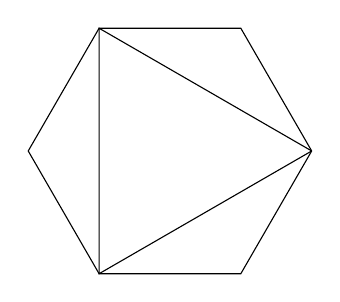
\begin{tikzpicture}[scale=.9]
  \newdimen\R
\R=2cm
  \draw (0:\R) \foreach \x in {60,120,...,360} { -- (\x:\R) } ;
  \draw (0:\R) \foreach \x in {120,240,360} { -- (\x:\R) } ;
\end{tikzpicture}
\caption{\label{fig:C3inC6}Geometrical shapes illustrating 
$\protect\CG_3$ as subgroup of $\protect\CG_6$.}
\end{marginfigure}

In order to obtain $\CG_3$ as a subgroup we can define
$F : \CG_6 \to \Set$ defined by $F(X,t) \defeq X/2$ for all $(X,t):\BCG_6$,
where $X/2$ is defined in \cref{sec:mthroot} as the quotient of $X$
modulo identifying elements that are an even power of $t$ away from each other.
Clearly, $F$ is a transitive $G$-set.
On symmetries, $F$ maps $\pi : (\bn6,\zs) \eqto (\bn6,\zs)$ to 
$([k] \mapsto [\pi(k)]) : (\bn6,\zs)/2 \eqto (\bn6,\zs)/2$.\footnote{%
The function $[k] \mapsto [\pi(k)]$ is well-defined since
permutations that commute with $\zs$ preserve distance.}
The symmetries $\pi$ satisfying $F(\pi)([0])=[0]$ are the
even powers of $\zs$.\footnote{%
In view of \cref{cor:id-m-cycle}, these symmetries can be visualized 
by the vertices of the regular triangle, see \cref{fig:C3inC6}.
The same is true for the symmetries picked out by $F(\pi)([1])=[1]$.
Both $F(\pi)([0])=[1]$ and $F(\pi)([1])=[0]$ give the other inscribed
regular triangle.} 
The subgroup that we have defined above is $(F,[0],!) : \Sub(\CG_6)$.
The underlying group of $(F,[0],!)$ is 
$\mkgroup(\sum_{(X,t):\Cyc_6} X/2, ((\bn6,\zs),[0]))$.
Using $\rho_2: \BCG_3 \ptdto \BCG_6$ from \cref{lem:deg-m-on-Cyc},
and the equivalence between $X/2$ and $\inv\rho_2 (X,t)$ from
\cref{thm:fiber-cdg}, and the equivalence from \cref{lem:sum-of-fibers},
we get an equivalence between the underlying group of  $(F,[0],!)$ and $\CG_3$.
\end{example}

There are other subgroups of $\CG_6$, and in this example they are accounted for simply by the various factorizations of the number $6$.

\subsection{Subgroups as monomorphisms}

%Three old para's that could still be useful as intro to this 
%A monomorphism into $G$ is given by a pointed connected groupoid  $\BH=(\BH_\div,\pt_H)$, a function $F:\BH_\div\to\BG_\div$ whose fibers are sets (a \covering) and an identification $p_f:\sh_G\eqto{}F(\sh_H)$.  There is really no need to specify that $\BH_\div$ is a groupoid: if $F:T\to \BG$ is a \covering, then $T$ is automatically a groupoid.

%On the other hand,  the type of \coverings over $\BG$ is equivalent to the type of $G$-sets: if $X:\BG\to\Set$ is a $G$-set, then the \covering is given by the first projection $\tilde X\to \BG$ where $\tilde X\defequi\sum_{y:\BG}X(y)$ and the inverse is obtained by considering the fibers of a \covering.  Furthermore, we saw in \cref{lem:conistrans} that $\tilde X$ being connected is equivalent to the condition $\istrans(X)$ of \cref{def:transitiveGset} claiming that the $G$-set $X$ is transitive.

%Hence, the type (set, really) $\typemono(G)$ of monomorphisms into $G$ is equivalent to the type of pointed connected \coverings over $\BG$, which again is equivalent to the type $\Sub(G)$ of transitive $G$-sets $X:\BG\to\Set$ together with a point in $X(\sh_G)$.

For many purposes it is useful to define ``subgroups'' slightly differently.
We now give a second, equivalent definition of a subgroup,
generalizing the examples $\dg{m}$ and $\cst{\base}$ from
the introduction of this chapter. Recall that both
$\USym\dg{m}$ and $\USym\cst{\base}$ are injective.
Also recall \cref{cor:fib-vs-path}\ref{set-fib-vs-path-point},
which implies that $\USymf$ is injective iff $\Bf$ is a \covering,
for any homomorphism $f$.

\begin{definition}
  \label{def:typeofmono}
  Let $G$ and $H$ be groups. We say that homomorphism $i: \Hom(H,G)$ is
  a \emph{monomorphism},\index{monomorphism} denoted $\ismono(i)$,
  %\glossary(isMono){$\protect{\ismono(i)}$}{proposition stating that
  %$i$ is a monomorphism of groups} gives error: culprit \ismono(i)?
  if $\USymi:\USymH\to \USymG$ is an injection  
  (all preimages of $\USymi$ are propositions).
  
  The \emph{type of monomorphisms into $G$}\footnote{%
  The similarity of this type with the type of subtypes
  $\Sub(T) \defeq \sum_{S:\UU}\sum_{f:S\to T}\isinj(f)$ in
  \cref{def:subtype} is not coincidental, and the remarks made 
  there in \cref{ft:incl-vs-inj} apply here as well.
  
  In particular, the identity type of $\typemono(G)$
  identifies precisely the triples that define the same subgroup,
  namely when their homomorphisms differ by precomposition by an 
  identification of their underlying groups.
  
  \MB{We should add in \cref{ch:absgroup} an equivalence between
  $\typemono(G)$ and the subsets of $\USymG$ with the usual closure
  properties --- the ultimate proof that we have the right 
  notion of concrete subgroup.}
  }
  \index{type! of monomorphisms into a group}
  \glossary(MonoG){$\protect{\typemono(G)}$}{type of monomorphisms%
  into the group $G$} 
  is
  \[
  \typemono(G)\defequi\sum_{H:\typegroup}\sum_{i:\Hom(H,G)}\ismono(i).
  \]
  
  We call $H$ the \emph{underlying group} of $(H,i,!) : \typemono(G)$.
  
  A monomorphism $(H,i,!)$ into $G$ is:
      \begin{enumerate}
      \item \emph{trivial}\index{trivial monomorphism} 
      if $H$ is the trivial group;\footnote{This amounts to $Bi$
      being the universal \covering over $BG$, see \cref{def:univ-cover}}
%.contractible (or, equivalently, if $\USymH$ is contractible),
      \item \emph{proper}\index{proper monomorphism} if $i$ is 
      not an isomorphism.\qedhere
      \end{enumerate}
\end{definition}
    
\begin{example}
  \label{ex:SGninSGn+1}
   \marginnote{
     That $i:\SG_2\to\SG_3$ is a monomorphism can visualized as follows:
     if $\SG_3$ represent all symmetries of an equilateral triangle in the
     plane (with vertices $1$, $2$, $3$), then $i$ is represented by the
     inclusion of the symmetries leaving $3$ fixed; \ie reflection through
     the line marked with dots in the picture.
\[ \begin{tikzpicture}[scale=.9]
  \newdimen\R
\R=2cm
  \newdimen\Rl
\Rl=2.3cm
  \draw (90:\R) \foreach \x in {210,330,450} { -- (\x:\R) } ;
  \node at (90:\Rl) {3};
  \node at (210:\Rl) {1};
  \node at (330:\Rl) {2};
  \draw[dotted] (90:\R) -- (270:\R * 0.5) ;
\end{tikzpicture}
\]}
We will present the subgroups from \cref{exa:fix1subSGn} with
monomorphisms. For each $n:\NN$, consider the  homomorphism 
$i_n:\Sigma_n\to\SG_{n+1}$ of permutation groups
with $\Bi_n$ sending $A:\BSG_n\defequi \FinSet_n$ to $A+\true:\BSG_{n+1}$.
As pointing path we take the reflexivity path.
This is a monomorphism since $\USymi_n:\USym\SG_n\to\USym\SG_{n+1}$ 
is an injection, extending any permutation $\pi$ of $\bn{n}$ to 
a permutation of $\bn{n}+\bn1$ by adding the last element as a
fixed point.

In the picture in the margin we have taken $n=3$ and
$\set{1,2,3}$ for $\bn{3}$. How can we obtain the other proper,
non-trivial subgroups of $\SG_3$? First of all, one should not
expect to find all subgroups through monomorphisms $j:\SG_2\to\SG_3$,
see \cref{xca:C3subSG3}. Using only $\SG_2$, the
two other subgroups can be obtained by varying the pointing
path of $i_3$. These pointing paths are induced by the permutations 
of $\bn{3}$. In \cref{xca:SG2subSG3} you are asked to elaborate each case.
\end{example}

\begin{xca}\label{xca:SG2subSG3}
Calculate $\im(\USymi_3)$ for each pointing path $\pi:\bn{3}\eqto\bn{3}$.
\end{xca}

\begin{xca}\label{xca:C3subSG3}
Define monomorphisms $j,j':\CG_3\to\SG_3$ such that $\USymj\neq \USymj'$
while $(\CG_3,j,!)$ and $(\CG_3,j',!)$ can be identified.
\end{xca}

\begin{example}
  \label{ex:prodinclismono}
  If $G$ and $H$ are groups, then $i_G : G \ptdto (G\times H)$ with
  $\Bi_G(z) \defeq (z,\sh_H)$, pointed by reflexivity, is a monomorphism:
  $\USymi_G$ maps $g:\USymG$ to $(g,\sh_H)$ and is obviously injective.
  We call $i_G$ the \emph{first inclusion} and we have a similar
  \emph{second inclusion} $i_H : H \ptdto (G\times H)$.
  % More generally, if $i:\Hom(H,G)$ is a homomorphism for which there (merely) exists a homomorphism $f:\Hom(G,H)$ such that $\id_H=fi$, then $i$ is a monomorphism.
  \end{example}


\begin{lemma}\label{lem:SubG=MonoG}
  Let $G$ be a group.
  The map sending $(X,\pt,!) : \Sub(G)$ to the monomorphism classified by  
  $\fst: (\sum_{z:\BG}X(z),(\sh_G,\pt))\ptdto\BG$, pointed by
  reflexivity, yields an equivalence\footnote{%
  Recall that we may omit "!"'s: propositional data never dies, 
  it just fades away!}
\[
F: \Sub(G)\to \typemono(G) : (X,\pt) \mapsto \Bigl(\mkgroup \bigl(\sum_{z:\BG}X(z),(\sh_G,\pt)\bigr),\mkgroup\fst\Bigr).\qedhere
\]
\end{lemma}

\begin{proof}
   The inverse equivalence is $E$ defined as follows:
 $$E:\typemono(G)\to\Sub(G),\qquad 
   (H,i)\mapsto E(H,i)\defequi (\Bi_\div^{-1},(\sh_H,\Bi_\pt)),$$
 %\glossary(E){$E$}{equivalence from $\typemono(G)$ to $\Sub(G)$}
  where the monomorphism $i:\Hom(H,G)$ is given by 
  the pointed map $(\Bi_\div,\Bi_\pt):\BH\ptdto\BG$.
  The preimage function $\Bi_\div^{-1}:\BG\to\Set$ is a transitive $G$-set 
  since $i$ is a monomorphism, and $(\sh_H,\Bi_\pt):\Bi_\div^{-1}(\sh_G)
  \defequi \sum_{x:\BH}(\sh_G\eqto{}\Bi_\div(x))$.
  Now do \cref{xca:SubG=MonoG} below.
\end{proof}

 \begin{example}\label{exa:EforSG3}
  In this example we explain how the equivalence between
  $\typemono(G)$ and $\Sub(G)$ works in the special case
  $G\jdeq\SG_3$ and with two versions of the same subgroup.
  
  Recall $(\SG_2,i_3,!):\typemono_{\SG_3}$ with
  $i_3: \SG_2\ptdto\SG_3 : B\mapsto (B+\true)$ from \cref{ex:SGninSGn+1}.
  The preimage function $\inv\Bi_3$ maps any $A:\BSG_3$
  to $\sum_{B:\BSG_2}(A\eqto{}(B+\true))$.
  In particular we have $(\bn2,\refl{\bn3}):\inv\Bi_3(\bn3)$
  (recall that $i_3$ is pointed by reflexivity).
   
  We have $E(\SG_2,i_3,!)\jdeq(\inv\Bi_3,(\bn2,\refl{\bn3}),!)$.
  Going back as in \cref{lem:SubG=MonoG} we get 
  $(\sum_{A:\BSG_3}\inv\Bi_3(A),\fst,!)$. Using \cref{lem:sum-of-fibers}
  one sees that, indeed, the latter monomorphism 
  can be identified with $(\SG_2,i_3,!)$.
  
  Why do we say that $(X_3,3,!):\Sub(\SG_3)$ from \cref{exa:fix1subSGn}
  defines the same subgroup as $(\SG_2,i_3,!):\typemono_{\SG_3}$
  from \cref{ex:SGninSGn+1}? The reason is that they pick out
  the same symmetries in $\SG_3$, as argued in these examples.
  Moreover, $(X_3,3,!)$ and $E(\SG_2,i_3,!)$ can be identified.
  Note that $X_3(A,!) \jdeq A$ and 
  $\inv\Bi_3 \jdeq \sum_{B:\BSG_2}(A\eqto{}(B+\true))$.
  Now apply \cref{xca:A-is-A-1+1} and verify that the points correspond.
  \cref{lem:E-preserves-symms} below offers a general result of this kind.
  \end{example}

\begin{xca}\label{xca:SubG=MonoG}
Complete the details of the proof of \cref{lem:SubG=MonoG} above using 
\cref{cor:fib-vs-path}\ref{set-fib-vs-path-point},
\cref{lem:sum-of-fibers},
\cref{lem:conistrans}.
\end{xca}

Since $\Sub(G)$ is a set by \cref{lem:SubGisset}, 
\cref{lem:SubG=MonoG} allows us to conclude:

\begin{corollary}\label{lem:setofsubgroups}
Let $G$ be a group. Then $\typemono(G)$ is a set.
\end{corollary}

The following lemma states that the equivalences in \cref{lem:SubG=MonoG} preserve the subsets of symmetries that are picked out.
\begin{lemma}\label{lem:E-preserves-symms}
  Let $G$ be a group and $g:\USymG$ a symmetry.
  Recall the equivalence $F$ from \cref{lem:SubG=MonoG}.
  For all $(X,\pt,!) : \Sub(G)$ and $(H,i,!) : \typemono(G)$
  such that $(H,i,!)=F(X,\pt,!)$,
  we have $X(g)(\pt) = \pt$ in $X_{\sh_G}$ if and only if 
  there exists $h:\USymH$ such that $g = \USymi(h)$ in $\USymG$.
\end{lemma}
\begin{proof}
Let $(X,\pt,!):\Sub(G)$. It suffices to prove the lemma for 
$(H,i,!)\jdeq F(X,\pt,!) : \typemono(G)$.
This means $\BH\jdeq(\sum_{z:\BG}X(z),(\sh_G,\pt))$ and $\Bi\jdeq\fst$.
We have to prove: $X(g)(\pt)=\pt$ iff there exists an
$h:(\sh_G,\pt)\eqto(\sh_G,\pt)$ such that $g = \USymi(h)\jdeq\loops\fst(h)$.

If $X(g)(\pt)=\pt$, then we can simply take $h\defeq(g,\refl{\pt})$.

For the converse, assume there exists an
$h:(\sh_G,\pt)\eqto(\sh_G,\pt)$ such that $g = \USymi(h)$.
Then $h = (g,p)$ for some $p: X(g)(\pt)=\pt$.\footnote{This path $p$ is
in fact equal to $\refl{\pt}$ since $X_{\sh_G}$ is a set.}
\end{proof}

\marginnote{%
  Which of the equivalent sets $\typemono(G)$ and $\Sub(G)$ is allowed to be called ``the set of subgroups of $G$'' is, of course, a choice.  It could easily have been the other way around and we informally refer to elements in either sets as ``subgroups'' and use the given equivalence $E$ as needed.
}%
\marginnote{%
  An argument for our choice can be
 as follows.  In set-based mathematics one has two options for defining "subgroup": either as a certain subset (uniquely given by its characteristic function to $\Prop$) or as an equivalence class of injections (taking care of size issues since the class of monomorphisms will not form a small set).  The former is the usual choice and is the one we model here with $\Sub(G)$, whereas the other corresponds to $\typemono(G)$.
  % that the identity type in $\Sub(G)$ seems more transparent than the one in $\typemono(G)$  (``more things are equal'' in $\typemono(G)$?), just as  $A\to\Prop$ gives more the intuition of picking out a subset by means of a characteristic function than what you get when considering the equivalent type of injections into $A$.
}


Through the equivalence $E$ we can translate the concepts in
\cref{def:typeofmono} to subgroups in $\Sub(G)$. 
First, observe that the underlying groups of a subgroup in $\typemono(G)$
and of its image under $E$ in $\Sub(G)$ can be identified.

\begin{definition}\label{def:triv-proper-Mono}
We say that a subgroup $(X,\pt,!):\Sub(G)$ is:
      \begin{enumerate}
      \item \emph{trivial}\index{trivial subgroup} if the underlying group
      $(\sum_{z:\BG}X(z),(\sh_G,\pt))$ is trivial;
      \item \emph{proper}\index{proper subgroup} if $X(\sh_G)$ is not
      contractible.\qedhere
      \end{enumerate}
\end{definition}
      
\begin{remark}\label{rem:notationsubgroup}
      A note on classical notation is in order.
If $(X,\pt,!)$ is a subgroup corresponding to a monomorphism $(H,i,!)$ into a group $G$, tradition would permit us to relax the burden of notation and we could write ``a subgroup $i:H\subseteq G$'', or, if we didn't need the name of $i:\Hom(H,G)$, simply ``a subgroup $H\subseteq G$'' or ``a subgroup $H$ of $G$''.
    \end{remark}
    
\begin{example}
  \label{ex:prodinclisGset}
  We saw in \cref{ex:prodinclismono} that the first 
  inclusion $i_1:G\to G\times G'$ is a monomorphism.
  The corresponding $G\times G'$-set is the composite of the first projection
  $\mathrm{proj}_1:\BG_\div\times\BG'_\div\to \BG_\div$ followed by the
  principal $G$-torsor $\princ G:\BG\to\Set: z\mapsto (\sh_G\eqto z)$ 
  of \cref{def:principaltorsor}.

  More generally, if $i:\Hom(H,G)$ and $f:\Hom(G,H)$, and $fi\eqto{}\id_H$,
  then $(H,i,!):\typemono(G)$, corresponding to the subgroup with $G$-set 
  given by the composite of $\Bf$ with the principal $H$-torsor $\princ H$.
\end{example}
    
    
\subsection{The Lagrange construction}

In this section we give a general version of Lagrange's Theorem.
It serves as a basis for more traditional versions, such as the
counting version in \cref{xca:lagrange} below.

\begin{construction}\label{con:lagrange}
Let $G$ be a group. For every subgroup $(X,\pt,!):\Sub(G)$ of $G$,
with underlying group called $H$, we have a function $L_H$ of type
\[
\bigl(\prod_{x:X(\sh_G)}\sum_{g:\USymG} g\cdot_X x = \pt \,\bigr) \to
\bigl(\USymG \eqto (X(\sh_G) \times \USymH)\bigr).
\]
\end{construction}

\begin{implementation}{con:lagrange}
Define the map $[\blank] : \USymG \to X(\sh_G)$ by $[g]\defeq g\cdot_X \pt$
for all $g:\USymG$. Then \cref{lem:sum-of-fibers} yields an
equivalence from $\USymG$ to the sum of fibers
$\sum_{x:X(\sh_G)}\inv{[x]}$.
For every $x:X(\sh_G)$, the fiber $\inv{[x]}$ of $[\blank]$ at $x$ is 
$\sum_{g:\USymG} (x = g\cdot_X \pt)$, and the latter subset
of $\USymG$ is equal to subset $(\sh_G,\pt)\eqto(\sh_G,x)$.
So we get an equivalence from $\USymG$ to 
$\sum_{x:X(\sh_G)}((\sh_G,\pt)\eqto(\sh_G,x))$. We are done if
we can replace this irritating little last $x$ with $\pt$, since
$\USymH\defeq((\sh_G,\pt)\eqto(\sh_G,\pt))$.
We use the premiss 
$\prod_{x:X(\sh_G)}\sum_{g:\USymG} (g\cdot_X x = \pt)$.
Applying \cref{xca:AC-in-TT} to this premiss, we obtain
a function $g:X(\sh_G)\to\USymG$ such that $g(x)\cdot_X x = \pt$
for all $x:X(\sh_G)$. In other words, $(g(x),!)$ is a path of type
$(\sh_G,x)\eqto(\sh_G,\pt)$, and hence postcomposition\footnote{%
\label{ft:lagrange-dep-sum}
Precomposition with the inverse gives an equivalence between
$(\sh_G,\pt)\eqto(\sh_G,x)$ and $(\sh_G,x)\eqto(\sh_G,x)$,
leading to the equivalence $L'_H$ in \cref{cor:lagrange-dep-sum}.}
gives the desired equivalence between $(\sh_G,\pt)\eqto(\sh_G,x)$ and 
$(\sh_G,\pt)\eqto(\sh_G,\pt)$. Thus we get in total an equivalence  
between $\USymG$ and $X(\sh_G) \times \USymH$, and we define $L_H(g)$
to be that equivalence.\footnote{This construction also works 
\inftygps acting on types. However, the premiss may be harder to
fulfill in such general cases.}
\end{implementation}

A minor modification of the above implementation,
indicated in \cref{ft:lagrange-dep-sum} gives \cref{cor:lagrange-dep-sum}, 
which is sometimes more convenient, \eg in the proof of \cref{lem:burnside}.

\begin{construction}\label{cor:lagrange-dep-sum}
Let conditions be as in \cref{con:lagrange}. Then
we have an equivalence $L'_H(f)$ between $\USymG$ and
$\sum_{x:X(\sh_G)}((\sh_G,x)\eqto(\sh_G,x))$.
\end{construction}

\begin{xca}\label{xca:lagrange}
The goal of this exercise is to state and prove the traditional
formulation of  Lagrange's Theorem. 
Let $G$ be a finite group and $(X,x,!):\Sub(G)$ a subgroup,
whose underlying group we call $H$. 
Assume that $X$ is a finite $G$-set. Show that $H$ is finite and
that $\Card(G) = \Card(X) \times \Card(H)$.
\end{xca}

\begin{xca}\label{xca:lagrange-Z-action-Rm}
The goal of this exercise is to illustrate that \cref{con:lagrange}
also can be applied to infinite groups. 
Recall the group of integers $\ZZ\jdeq\mkgroup{(\Sc,\base)}$ and the $\ZZ$-set
$R_m: \Sc\to\Set$ from \cref{def:RmtoS1}, defined by $R_m(\base) \defeq \bn m$
and $R_m(\Sloop) \defis \zs$, for $m>0$. Let $H_m$ be the underlying group
of $(R_m,0,!)$. Identify $\USym\ZZ$ with $\bn m \times \USymH_m$.
\end{xca}

\begin{xca}\label{xca:lagrange-if-subgr-not-normal}\MB{TBD: }
The goal of this exercise is to illustrate that \cref{con:lagrange}
also can be applied to infinite groups and a subgroup that is "abnormal".
Recall \cref{fig:not-normal} ...
\end{xca}





    % commented out by BID 211117 Some examples and references should be included when the cyclic subgroups are fully developed
    % \subsection{The geometry of subgroups: some small examples}\footnote{this subsection is not touched: it needs attention}
% \label{smallsubgpex}

% As a teaser, and in order to get a geometric feel for the subgroups and their intricate interplay, it can be useful to have some fairly manageable examples to stare at.
% Some of the main tools for analyzing the geometry of subgroups are collected in \cref{sec:fingp} on finite groups, and we hope the reader will be intrigued by our mysterious claims and go on to study \cref{sec:fingp}.
% That said, the examples we'll present are possible to muddle through by hand without any fancy machinery, but brute force is generally not an option and even for the present examples it is not something you want to show publicly.

% When presenting the subgroups of a group $G$, three types are especially revealing: the set of subgroups $\Sub(G)(\sh_G)$, the \emph{groupoid of subgroups} $\typesubgroup(G)\defequi\sum_{y:\BG}\Sub(G)(y)$ and what we for now call the ``set of normal subgroups'' $\prod_{y:\BG}\Sub(G)(y)$.   Our local use of ``normal subgroup'' is equivalent to the official definition to come.

% The first projection $\typesubgroup(G)\to \BG$ is referred to as the \emph{\covering of subgroups}.

% \footnote{Write out and fix the concrete examples (cyclic groups and $\Sigma_3$) commented out}
% % \begin{remark}
% % In  \cref{cha:circle} we studied the subgroups of the group of integers $G\eqto{}\ZZ$ through \coverings over the circle $S^1$ (which we showed was equivalent to $B\ZZ$).
% % We discovered a subgroup $n\ZZ$ for each natural number $n:\NN$ and in the groupoid $\typesubgroup({\ZZ})$ these sit as elements in separate components.  Each of these components are contractible (because addition is commutative: $\ZZ$ is an abelian group).

% % In general, a component $K$ of the groupoid $\sum_{y:\BG}\Sub(G)(y)$ of subgroups of a group $G$ may be much more interesting. For one thing the, $K$ can contain many subgroups in the sense that the preimage of the first projection $K\to \BG$ is a set that may have many different elements; each representing a subgroup.  However, this set of subgroup will be a \emph{conjugacy class} of subgroups: the different subgroups are related by the conjugation action of $G$.

% % If $G$ is abelian this action is trivial, and $\sum_{y:\BG}\Sub(G)(y)$ consists of contractible components indexed over the subgroups of $G$.  Otherwise different subgroups may live in the same component of the groupoid of subgroups -- we'll see examples in a moment.

% % In addition, the components will not in general be contractible, revealing the symmetries of the subgroups under the conjugation action.
% % \end{remark}


% % \begin{example}
% %   The trivial group only has itself as a subgroup; the groupoid of subgroups and the set of normal subgroups are singletons.
% % \end{example}
% % \begin{example}
% %   The cyclic group $C_p$ of prime order $p$ has only two subgroups, the trivial and the full subgroup itself and both are normal.  In fact, all subgroups of abelian groups are normal.

% % In general, the cyclic group $C_n$ of order $n$ has exactly one subgroup for each divisor $i$ of $n$.
% % \end{example}


% % \begin{example}
% %   The group $C_2\times C_2$ has has no less than five subgroups: the trivial one, three subgroups that as groups (as opposed as \emph{sub}groups) are equivalent to $C_2$ and the full group $C_4$ itself.
% % \end{example}
% % \begin{remark}
% %   The permutation group $\Sigma_3$ has four nontrivial proper subgroups.  Three conjugate subgroups isomorphic as groups to $C_2$ and one normal one which is as a group is isomorphic to $C_3$.  The component containing the copies of $C_2$ is equivalent to a circle.
% % \end{remark}

\section{Invariant maps and orbits}
\label{sec:fixpts-orbits}
We now return to some important constructions involving $G$-sets 
for a group $G$.
Some of these make equally good sense for \emph{$G$-types} for \aninftygp
$G$, in which case we add a footnote to this effect.

We are particularly interested in what happens when a $G$-set
is not transitive, that is, does not satisfy the requirement of 
\cref{def:transitiveGset}. In \cref{cha:circle}, under the name
of \coverings over the circle, we have already seen examples of
transitive and non-transitive $\Sc$-sets:
In \cref{fig:covering} the left picture exhibits a transitive one,
and the right picture  a non-transitive one. Also, 
\cref{fig:two-comp-S1-cover} shows a non-transitive $\Sc$-set,
whereas the $m$\th power bundle over the circle in
\cref{fig:m-th-power} is a transitive $\Sc$-set.
\cref{lem:conistrans} gives a good explanation of these pictures:
A $G$-set is transitive if and only if the associated \covering is connected.
In other words, if a $G$-set $X:\BG\to\Set$ is transitive, then the
group action connects\footnote{In the sense that $\Trunc{(z,x)\eqto(w,y)}$
if and only if there exists a $g:z\eqto w$ such that $g\cdot_X x = y$.} 
any two elements in the total type $\sum_{x:\BG} X(z)$.
If $X$ is not transitive, then the latter total type falls apart 
in different components. Since these components are themselves
connected, the choice of an element of them gives rise to a subgroup of $G$
in the sense of \cref{def:set-of-subgroups}.

% perhaps with some warnings $\USymG$, $=$, \cref{lem:conistrans}, ...
\begin{definition}\label{def:actiontype} 
  Let $G$ be a group and $X : \BG\to\Set$ a $G$-set,\footnote{%
  This definition can be generalized to \inftygps $G$ and $G$-types $X$.}
  then the \emph{action type}\index{action type}
  of $X$, denoted\footnote{%
    The superscripts and subscripts are decorated with ``$hG$'',
    following a convention in homotopy theory.
    The action type is sometimes denoted $X \dblslash G$.}
\[
  X_{hG} \defeq \sum_{z:\BG} X(z),
\]
is the total type of $X$, see \cref{sec:sum-types}.
By \cref{def:pathover-trp} and \cref{def:pairtopath},
we get an equivalence
\[
\bigl((z,x)\eqto_{X_{hG}}(w,y)\bigr) \equivto
\sum_{g:z\eqto w} g\cdot x = y,
\]
which also goes for their (often used) propositional truncations.
%We use $(z,y):X_{hG}$ sometimes for $z:\BG,\,y:X(z)$.

The type of \emph{invariant maps}\footnote{%
Invariant maps are dependent functions $f$ and the reason for the new name
in this context is that $f(z) = g \cdot_X f(z)$ for any $z:\BG$
and $g:z\eqto z$. Cf.~\cref{lem:fixed-char}. Note that there need not 
be any invariant maps: $\prod_{z:\Sc}\base\eqto z$ is empty.
Using \cref{lem:univisexp}, \cref{fig:transportalongloop} explains
why: the successor function has no fixed point.
}
\index{invariant map type} is
\[
  X^{hG} \defeq \prod_{z:\BG} X(z).
\]

The \emph{set of orbits} (soon to be identified with the
set truncation of $X_{hG}$, see \cref{lem:X/G=setTruncX_hG})
\index{set!of orbits}\index{orbit set} is the subset of $\Sub_G(X)$ consisting
of all $G$-subsets $P$ of $X$ such that the underlying $G$-subset $X_P$
is transitive:\footnote{See \cref{def:transitiveGset}.}
\[
  X / G \defeq \sum_{P:\Sub_G(X)}\istrans(X_P).\qedhere
\]
\end{definition}

We have seen many instances of action types before:
When $G$-sets are considered as \coverings $f : A \to \BG$,
they are the domains $A$.
Recall for example~\cref{fig:two-comp-S1-cover},
showing an action of $\ZZ$ on $\set{1,2,3,4,5}$ with no invariant maps
and an action type equivalent to a sum of two circles.
In~\cref{fig:ZZ-set-orbits}, we show a similar $\ZZ$-set,
with underlying set $\set{0,1,2,3,4,5}$, three orbits,
and $5$ corresponding to the only invariant map.\footnote{%
Sending $\base$ to $5$ and $\Sloop$ to $\refl{5}$.}

\begin{marginfigure}
  \begin{tikzpicture}[scale=.15]
    \node (Sc) at (0,-5) {$\B\ZZ$};
    \node[dot,label=left:$5$] (five)   at (-10,30) {};
    \node[dot,label=left:$4$] (four)   at (-10,22) {};
    \node[dot,label=left:$3$] (three)  at (-10,18) {};
    \node[dot]                (base)   at (-10,-5) {};
    \node[label=left:$\Sloop$] (Sloop) at (10,-5) {};

    \pgfmathsetmacro\cc{.55228475}% = 4/3*tan(pi/8)
    \pgfmathsetmacro\cy{2*\cc}%
    \pgfmathsetmacro\cx{10*\cc}%
    \pgfmathsetmacro\intx{3.5}%
    \pgfmathsetmacro\inty{1.5}%
    \pgfmathsetmacro\ay{.35165954}%

    \draw (-10,18) .. controls (-10,18 - \cy + \ay) and (-\cx,17 - \ay)
    .. (0,17) .. controls (\cx,17 + \ay) and (10,20 - \cy - \ay) .. (10,20)
    .. controls (10,20 + \cy + \ay) and (\cx,23 - \ay)
    .. (0,23) .. controls (-\cx,23 + \ay) and (-10,22 + \cy - \ay)
    .. (-10,22) .. controls (-10,22 - \cy + \ay) and (-\cx,21 - \ay)
    .. (0,21) .. controls (\cx,21 + \ay) and (10,24 - \cy - \ay)
    .. (10,24)
    .. controls (10,24 + \cc) and (\intx + \cx, 24 + \inty + \ay)
    .. (\intx,24 + \inty) .. controls (\intx - \cx,24 + \inty - \ay)
    and (-\intx + \cx,20 + \ay)
    .. (-\intx,18 + \inty) .. controls (-\intx - \cx,18 + \inty - \ay)
    and (-10,18 + \cc) .. (-10,18);
    \draw[casblue] (-10,2) .. controls (-10,2 - \cy + \ay) and (-\cx,1 - \ay)
    .. (0,1) .. controls (\cx,1 + \ay) and (10,4 - \cy - \ay)
    .. (10,4)
    \foreach \y in {4,8} {
      .. controls (10,\y + \cy + \ay) and (\cx,3 + \y - \ay)
      .. (0,3 + \y) .. controls (-\cx,3 + \y + \ay) and (-10,2 + \y + \cy - \ay)
      .. (-10,2 + \y) .. controls (-10,2 + \y - \cy + \ay) and (-\cx,1 + \y - \ay)
      .. (0,1 + \y) .. controls (\cx,1 + \y + \ay) and (10,4 + \y - \cy - \ay)
      .. (10,4 + \y) }
    .. controls (10,12 + \cc) and (\intx + \cx, 12 + \inty + \ay)
    .. (\intx,12 + \inty) .. controls (\intx - \cx,12 + \inty - \ay)
    and (-\intx + \cx,4 + \ay)
    .. (-\intx,2 + \inty) .. controls (-\intx - \cx,2 + \inty - \ay)
    and (-10,2 + \cc) .. (-10,2);
    \draw (10,-5) .. controls ++(0,\cy) and ++(\cx,0)
    .. (0,-3) .. controls ++(-\cx,0) and ++(0,\cy)
    .. (-10,-5) .. controls ++(0,-\cy) and ++(-\cx,0)
    .. (0,-7) .. controls ++(\cx,0) and ++(0,-\cy) .. (10,-5);

    \draw (10,30) .. controls ++(0,\cy) and ++(\cx,0)
    .. (0,32) .. controls ++(-\cx,0) and ++(0,\cy)
    .. (-10,30) .. controls ++(0,-\cy) and ++(-\cx,0)
    .. (0,28) .. controls ++(\cx,0) and ++(0,-\cy) .. (10,30);

    \node[dot,label=left:$2$,casred] (two)   at (-10,10) {};
    \node[dot,label=left:$1$,casred] (one)   at (-10, 6) {};
    \node[dot,label=left:$0$,casred] (zero)  at (-10, 2) {};
  \end{tikzpicture}
  \caption{A $\ZZ$-set with three orbits and one invariant map.}
  \label{fig:ZZ-set-orbits}
\end{marginfigure}

In~\cref{fig:ZZ-set-orbits} we have highlighted one single component of
the action type in blue (\ie corresponding to an element of the set of orbits),
and we see that it contains a subset of the underlying set,
the three red elements $\set{0,1,2}$.
Such a set is what is traditionally called an orbit.
This connection is emphasized in \cref{cor:orbit-equiv}.

\begin{definition}\label{def:orbit-map}
Let $G$ be a group and $X : \BG\to\Set$ a $G$-set.
We define the map $[\blank]_0$ from the action type $X_{hG}$ of
$X$ to $\Sub_G(X)$, the set of $G$-subsets of $X$, as follows.
For any $u:X_{hG}$, let $[u]_0$ be the $G$-subset of $X$ that
sends $z:\BG$ to
\[
(x:X(z) \mapsto \Trunc{u\eqto(z,x)}) : X(z) \to \Prop.\qedhere
\]
\end{definition}

Recall from \cref{def:actiontype} the equivalence of
$\Trunc{(z,x)\eqto(w,y)}$ and $\exists_{g:z\eqto w}(g\cdot x = y)$.
The next lemma follows easily from the properties of $\Trunc{u\eqto(z,x)}$.

\begin{lemma}\label{lem:[]0-maps-to-X/G}
Let $G$ be a group and $X : \BG\to\Set$ a $G$-set.
For every $u:X_{hG}$, the underlying $G$-set
$(z\mapsto \sum_{x:X(z)}\Trunc{u\eqto(z,x)})$ of $[u]_0$,
defined in \cref{def:Gsubset}, is transitive.
Hence $[\blank]_0$ is a map from $X_{hG}$ to $X/G$.
\end{lemma}

In view of the above lemma, we call $[u]_0$ \emph{the orbit
through} $u$. \glossary(orbit){$[u]_0$}{orbit through $u:X_{hG}$}
The following lemma implies that the set of orbits can 
be identified with the set truncation of the action type.

\begin{lemma}\label{lem:X/G=setTruncX_hG}
  Let $G$ be a group and $X : \BG\to\Set$ a $G$-set.\footnote{%
  This lemma can be generalized to \inftygps $G$ and $G$-types $X$.}
  Then the map $[\blank]_0 :X_{hG}\to X/G $ is surjective.
  Moreover, we have a (unique) identification of
  $(X/G,[\blank]_0)$ and $(\setTrunc{X_{hG}},\settrunc{\blank})$
  in the type $\sum_{S:\Set}(X_{hG}\to S)$.
\end{lemma}

\begin{proof}
  Consider an orbit $O:X/G$, \ie
  $O$ is a $G$-subtype of $X$ such that $X_O$ is transitive. 
  We have to show that there exists a $u:X_{hG}$ such that $O=[u]_0$.
  By the connectivity of $\BG$ it suffices to show 
  $O(\sh_G)=_{X(\sh_G)\to\Prop}[u]_0(\sh_G)$ for some $u$.
  Transitivity of $X_O$ means that there exists an $x:X(\sh_G)$
  such that $O(\sh_G,x)$ and for all $y:X(\sh_G)$ such that
  $O(\sh_G,y)$ there
  exists a $g:\USymG$ such that $g\cdot x = y$, \ie $[(\sh_G,x)]_0(\sh_G,y)$.
  So we take $u\defeq(\sh_G,x)$ and have to show $O(\sh_G,y)$ if and only if
  $[u]_0(\sh_G,y)$, for all $y:X(\sh_G)$. But this follows directly from
  the observation made just above the lemma
  (see also \cref{rem:equivalents-of-[x]=[y]} below).
  
  The second part of the lemma follows from \cref{rem:set-trunc-as-quotient}. 
\end{proof}

Another way to state the above lemma is that the map 
$[\blank]_0 :X_{hG}\to X/G$ factors as the composite of $\settrunc\blank$
followed by a unique equivalence: $X_{hG}\to \setTrunc{X_{hG}}\equivto X/G$.

\begin{corollary}\label{cor:orbit-equiv}
Define the map $[\blank] : X(\sh_G) \to X/G$ by $[x]\defeq[(\sh_G,x)]_0$.
Then $[\blank]$ is surjective and induces
by \cref{xca:map-induces-quotient}\ref{it:surj-ind-quot=codomain}
an equivalence between the induced quotient of $X(\sh_G)$ and $X/G$.
Moreover, $[x] = [y]$ is equivalent to $\exists_{g:\USymG}(g\cdot x = y)$.
\end{corollary}

In view of this corollary, we call $[x]$ \emph{the orbit
through} $x$. \glossary(orbit){$[x]$}{orbit through $x:X(\sh_G)$}
\begin{proof}
In the proof of surjectivity in \cref{lem:X/G=setTruncX_hG} we used
$u\defeq(\sh_G,x)$ to get $O=[u]_0$, so $[\blank]$ is surjective. 
The last statement follows since
both propositions are equivalent to $\Trunc{(\sh_G,x)\eqto(\sh_G,y)}$.
\end{proof}

\begin{remark}\label{rem:SubGX=Sub(X/G)}
Let $G$ be a group and $X : \BG\to\Set$ a $G$-set.
We have the following chain of definitions and equivalences:
\begin{align*}
\Sub_G(X)&\jdeq \prod_{z:\BG}(X(z)\to\Prop) 
\\
         & \we \bigl(X_{hG}\to\Prop\bigr)
               \quad\text{(by \cref{ft:SubTotX,xca:Sigma-curry})}
\\
         & \we \bigl(\setTrunc{X_{hG}}\to\Prop\bigr) 
               \quad\text{(since $\Prop$ is a set)}
\\        
         & \we \bigl(X/G\to\Prop\bigr)
               \quad\text{(by \cref{lem:X/G=setTruncX_hG})}
\\
         & \jdeq \Sub(X/G).\qedhere
\end{align*}
\end{remark}

\begin{xca}\label{xca:transX-just1orbit}
Show: $X/G$ is contractible if and only if $X$ is transitive.
%That $X/G$ is contractible encodes that there is just one orbit.
%Hint: use \cref{lem:conistrans}.
\end{xca}


\begin{remark}\label{rem:equivalents-of-[x]=[y]}
Given a group $G$, a $G$-set $X$ and $x,y:X(\sh_G)$,
the following propositions are all equivalent and we may pass from
one to another without mention:
\begin{itemize}
\item $[x]=_{X/G}[y]$;
\item $[x](\sh_G)=_{X(\sh_G)\to\Prop}[y](\sh_G)$;
\item $\exists_{g:\USymG}(g\cdot x = y)$;
\item $\Trunc{(\sh_G,x)\eqto(\sh_G,y)}$;
\item $[x](\sh_G,y)$;
\item $[y](\sh_G,x)$.
\end{itemize}
As functions of $x$ and $y$, all of the above define the equivalence
relation on $X(\sh_G)$ induced by the surjection $[\blank]$. 
\end{remark}

Thus, both the underlying set $X(\sh_G)$ and the action type
$X_{hG}$ have equivalence relations (induced by the surjections $[\blank]$
and $[\blank]_0$, respectively) with quotient set $X/G$.\footnote{%
  \label{ft:orbit-surj}
  This also justifies the notation $X/G$.
  We have a diagram of surjective maps:
  \[
    \begin{tikzcd}[ampersand replacement=\&]
      X(\sh_G) \ar[rr,"{x\mapsto(\sh_G,x)}"]\ar[dr,"{[\blank]}"']
      \& \& X_{hG}\ar[dl,"{[\blank]_0}"] \\
      \& X/G \&
    \end{tikzcd}
  \]}
  We can write $X(\sh_G)$ and $X_{hG}$ as sums of the respective fibers,
  which we will elaborate in the next paragraphs.

Let $O:X/G$ be an orbit and consider 
$\inv{[O]_0} \jdeq \sum_{u:X_{hG}}(O=[u]_0)$. Note that
the underlying $G$-set $X_O\jdeq(z:\BG \mapsto \sum_{y:X(z)}O(z,y))$
of $O$ is transitive. It follows that
$O(u)$ holds if and only if $O=[u]_0$, for all $u:X_{hG}$.%
\footnote{We use the first step of \cref{rem:SubGX=Sub(X/G)}.
If $O(u)$ and $O(v)$, then $\Trunc{u\eqto v}$
by the transitivity of $X_O$. The rest is obvious.} 
Therefore, the fiber $\inv{[O]_0}$ is equivalent to the action type
$(X_O)_{hG}\jdeq\sum_{z:\BG} X_O(z)$.

After the previous paragraph, the elaboration of 
$\inv{[O]} \jdeq \sum_{x:X(\sh_G)}(O=[x])$ is easy.
Recall that $[x]\jdeq[(\sh_G,x)]_0$, so that the fiber $\inv{[O]}$
is equivalent to the underlying set of $X_O$, \ie
$X_O(\sh_G)\jdeq\sum_{x:X(\sh_G)} O(\sh_G,x)$
via identity on first components.
We depict the situation in the diagram%
\footnote{\label{ft:orbit-fibs}%
Along the horizontal arrow, $(O,x)$ maps to $(O,(\sh_G,x))$, for $x:X_O(\sh_G)$.
  \[
    \begin{tikzcd}[ampersand replacement=\&,column sep=tiny]
      \displaystyle\sum_{O:X/G} X_O(\sh_G) \ar[rr]\ar[dr,"\fst"']
      \& \& \displaystyle\sum_{O:X/G} (X_O)_{hG}\ar[dl,"\fst"] \\
      \& X/G \&
    \end{tikzcd}
  \]
}
in the margin. Note how the role of $X$ in \cref{ft:orbit-surj} 
is taken over by $X_O$. 

\begin{definition}\label{def:orbit-stabilizer}
  Let $G$ be a group, $X : \BG \to \Set$ a $G$-set, 
  and $x : X(\sh_G)$ an element.\footnote{%
  This definition can be generalized to \inftygps $G$ and $G$-types $X$.}
  \begin{enumerate}
  \item Define the group $G_x \defeq \Aut_{X_{hG}}(\sh_G,x)$.
% $(\sum_{z:\BG}\sum_{y:X(z)}\Trunc{(\sh_G,x) \eqto (z,y)},(\sh_G,x,!))$.
  Clearly, $\fst:\BG_x \to \BG$ is a set bundle:
  each fiber at $z:\BG$ is a subset of $X(z)$.
  Hence $(G_x,\fst,!):\typemono(G)$ is monomorphism into $G$.
  We call the subgroup $G_x$ of $G$ the 
  \emph{stabilizer (sub)group}\index{stabilizer}%
    \index{group!stabilizer} at $x$. The inclusion $\fst$ of $\BG_x$ in
    $\BG$ classifies a monomorphism denoted by $i_x : \Hom(G_x,G)$.
  \item Define $G\cdot x \defeq \setof{y : X(\sh_G)}{[x] =_{X/G} [y]}$
    to be the \emph{underlying set of the orbit through $x$}.\footnote{%
    This is short for the underlying set of the underlying $G$-set of the
    orbit $[x]$ of $X$.}
    \qedhere
  \end{enumerate}
\end{definition}

\begin{remark}\label{rem:orbit-fibs}
In the above definition, the underlying $G$-set $X_{[x]} \jdeq
(z:\BG)\mapsto\sum_{y:X(\sh_G)}\Trunc{(\sh_G,x)\eqto(z,y)}$
of the orbit $[x]$ plays an important double role: On one hand its
action type $(X_{[x]})_{hG}$,
%$\sum_{z:\BG}\sum_{y:X(z)}\Trunc{(\sh_G,x)\eqto(z,y)}$,
pointed at $(\sh_G,x)$, is the classifying type $\BG_x$ of the stabilizer
group $G_x$. On the other hand it is a transitive $G$-set whose
underlying set $\sum_{y:X(\sh_G)}\Trunc{(\sh_G,x)\eqto(\sh_G,y)}$
is the underlying set of the orbit $[x]$. Thus,
for $O\jdeq[x]$, we have easy identifications of $G\cdot x$ and $X_O(\sh_G)$,
as well as of $\BG_x$ and $(X_O)_{hG}$, using $[x]\jdeq[(\sh_G,x)]_0$.
Applying the maps in \cref{ft:orbit-fibs} in this particular case, 
we obtain \cref{fig:fibs-at-[x]}.
\begin{marginfigure}
  \[\footnotesize %MB20250324: footnotesize should be default
    \begin{tikzcd}[ampersand replacement=\&,column sep=tiny]
      ([x], y) \ar[rr,mapsto]\ar[dr,mapsto,"\fst"']
      \& \& ([(\sh_G,x)]_0,(\sh_g,y))\ar[dl,mapsto,"\fst"] \\
      \& {[x]} \&
    \end{tikzcd}
  \]
  \caption{\label{fig:fibs-at-[x]}Along the horizontal arrow,
  the second component $y:G\cdot x$ is mapped to $(\sh_g,y):\BG_x$.}
\end{marginfigure}

Note furthermore that the base point of $\BG_x$ depends on the choice of $x$,
but the underlying type $(\BG_x)_\div$, being a connected component,
only depends on the orbit $[x]:X/G$.
\end{remark}

\begin{xca}\label{xca:[x]=[y]-implies-||Gx=Gy||}
Let $G$ be a group and $X: \BG\to\Set$ a $G$-set. Show:
if $[x]=[y]$, then $\Trunc{G_x\eqto G_y}$, for any $x,y:X(\sh_G)$.
%Solution: conclusion is prop, so we may assume we have a $g:\USymG$
%such that $g\cdot x = y$. Hence we have $p: (\sh_G,x)\eqto(\sh_G,y)$,
%so $\BG_x\eqto\BG_y$ by application on this path $p$.
\end{xca}

\begin{remark}\label{rem:subgrp-is-stabsubgr}
  In fact every subgroup of $G$ is a stabilizer subgroup.
  We can equivalently define the stabilizer subgroup of $x$ 
  by an element of $\Sub(G)$, namely
  the transitive $G$-set $X_{[x]}$, pointed by
  $x$ as element of the subset $X_{[x]}(\sh_G)$ of $X(\sh_G)$.
  If $X$ is transitive, then all orbits are equal (\cref{xca:transX-just1orbit})
  and the stabilizer subgroup of $x$ simplifies to $(X,x,!):\Sub(G)$,
  a general form defining a subgroup of $G$.
\end{remark}

The following lemma states that the orbits of a $G$-set $X$
sum up to its underlying set, with the sum taken over the set
of orbits $X/G$.

\begin{lemma}
  \label{lem:splitting into orbits}
  The inclusions of the orbits form an equivalence
\[
  (O,x,!)\mapsto x \quad:\quad
  \bigl(\sum_{O:X/G} \inv{[O]} \bigr) \we X(\sh_G).
\]
\end{lemma}
\begin{proof}
Recall that $\inv{[O]}\jdeq \sum_{x:X(\sh_G)}(O=[x])$, 
and then abstract
away the $O$ using \cref{lem:contract-away}.\footnote{%
In fact, for every set $A$ and every equivalence relation on $A$,
the equivalence classes sum up to $A$.}
\end{proof}

There are two possible extreme cases for $G_x$ that are important:
\begin{definition}\label{def:fixed-free}
  Let $G$ be a group, $X$ a $G$-set and $x:X(\sh_G)$ an element of the underlying set.\footnote{%
  This definition can be generalized to \inftygps $G$ and $G$-types $X$.}
  We say that
  \begin{enumerate}
  \item $x$ is \emph{fixed}\index{fixed}
    if $i_x$ is an isomorphism (so $G_x$ is all of $G$), and
  \item $x$ is \emph{free}\index{free}\index{action!free}
    if $G_x$ is trivial.
  \end{enumerate}
  We say that $X$ itself is \emph{free} if each $x:X(\sh_G)$ is free.
\end{definition}

\begin{example}\label{exa:fixed-free-neither}
Let $G$ be a group. For every set $S$, every element $s:S$ is fixed
under the trivial $G$-set $\triv_G S$, since the group action is the 
identity function. In contrast,
every element $g:\USymG$ is free under the $G$-set 
$\princ G \jdeq(\sh_G \eqto \blank)$, 
as $\sum_{z:\BG}\princ G(z))$ is contractible.
For an example with more variation, see \cref{exa:prep-burnside} upto
\cref{fig:C4-action-on-4-bits}. Find the fixed elements, the free elements
and those that are neither fixed nor free.
\end{example}

\begin{xca}\label{xca:fixed-free-neither}
Make sure you understand \cref{exa:fixed-free-neither} by
elaborating:
\begin{itemize}
\item $\BG_s$ in the case of $\triv_G S$,
\item $\BG_g$ in the case of $\princ G$, 
\item $\BG_f$ for each $f:\bn4\to\bn2$
in the case of \cref{exa:prep-burnside}, see \cref{fig:C4-action-on-4-bits}.
\end{itemize}
\end{xca}

\begin{lemma}\label{lem:free-pt-char}
  Let $G$ be a group and $X$ a $G$-set. Then we have for all $x:X(\sh_G)$
  that $x$ is free if and only if the (surjective) map
  $(\blank \cdot x) : \USymG \to (G\cdot x)$ is injective
  (and hence a bijection).
\end{lemma}
\begin{proof}
  Consider two elements of the orbit, say $g\cdot x,g'\cdot x$ for $g,g':\USymG$.
  We have $g\cdot x=g' \cdot x$ if and only if $x = \inv{g} g'\cdot x$
  if and only if $\inv{g} g'$ lies in $\USymG_x$.
  Hence the map $(\blank \cdot x)$ is injective iff $\USymG_x$ is contractible.
  Now use \cref{xca:connected-trivia} yielding that that 
  $G_x$ is trivial iff $\USymG_x$ is contractible.
\end{proof}

\begin{lemma}\label{lem:X_hG-set-iff-Xfree}
Let $G$ be a group and $X:\BG\to\Set$ a $G$-set.\footnote{%
This lemma can be generalized to \inftygps $G$ and $G$-types $X$.}
Then the following propositions are equivalent:
\begin{enumerate}
\item The action type $X_{hG}$ is a set;
\item The map $[\blank]_0 :X_{hG}\to X/G$ from 
      \cref{def:orbit-map} is an equivalence;
\item The $G$-set $X$ is free.
\end{enumerate}
\end{lemma}
\begin{proof}
We prove the relevant implications in circular order.
\begin{enumerate}
\item Assume $X_{hG}$ is a set. The map  $[\blank]_0 :X_{hG}\to X/G$ is
surjective by \cref{lem:X/G=setTruncX_hG}, so it suffices to show
it is injective. Since $X_{hG}$ is a set, it suffices to
show that $[u]_0=[v]_0$ implies $u=v$, for all $u,v:X_{hG}$.
This follows immediately from the definition of $[\blank]_0$, 
as the propositional truncation plays no role.
\item Assume $[\blank]_0 :X_{hG}\to X/G$ is an equivalence.
Then $X_{hG}$ is a set since $X/G$ is a set, and hence
all components of $X_{hG}$ are contractible.
It follows that all stabilizer groups $G_x$ are trivial,
and hence $X$ is free.
\item Assume $X$ is free. Then all stabilizer groups $G_x$ are trivial,
so all identity types $(\sh_G,x)\eqto (\sh_G,x)$ are contractible.
Since $\BG$ is connected we get that $u\eqto u$ is contractible
for all $u:X_{hG}$. Hence $X_{hG}$ is a set.\footnote{%
A type $T$ is a set 
if and only if all identity types $t\eqto_T t$ are contractible.}\qedhere
\end{enumerate}
\end{proof}

\begin{lemma}\label{lem:fixed-char}
  Given a group $G$ and a $G$-set $X$, an element $x:X(\sh_G)$ is
 fixed if and only if the orbit $G\cdot x$ is contractible,
  \ie $x = g\cdot x$ for all $g:\USymG$.\footnote{%
  This lemma can be generalized to \inftygps $G$ and $G$-types $X$.
  In that case $\USymG\defeq\loops\BG$ is the underlying \emph{type} of $G$.}
\end{lemma}
\begin{proof}
  The orbit $G\cdot x$ of $x$ is the fiber of $\Bi_x : \BG_x \ptdto \BG$
  at $\sh_G$. Since $\BG$ is connected,
  this is contractible if and only if all fibers of $\Bi_x$ are contractible,
  \ie $\Bi_x$ is an equivalence, which in turn is equivalent to $i_x$
  being an isomorphism.
\end{proof}

When $X : \BG \to \Set$ is a $G$-set for an ordinary group $G$, the subset
\[
  \setof{x : X(\sh_G)}{\text{$x$ is fixed}}
\]
is closely related to the type $X^{hG}$ of invariant maps.
If we evaluate an invariant map $f : \prod_{z:\BG}X(z)$ at $\sh_G$
we do indeed land in this subset:
Letting $x\defeq f(\sh_G)$,
and taking the dependent action on paths,
$\apd{f}(g) : \pathover x X g x$,
we can use~\cref{def:pathover-trp} to conclude
$\trp[X] g(x)\jdeq g\cdot x = x$, for all $g:\USymG$.
The following lemma states that, conversely, each fixed $x$ uniquely
determines an invariant map.

\begin{lemma}\label{lem:fixpts-are-fixed}
  Let $G$ be a group and $X$ a $G$-set,\footnote{\MB{%
  We use the connectivity of $\BG$ and that $X(\sh_G)$ is a set.}}
  with $X^{hG} \jdeq \prod_{z:\BG}X(z)$
  the set of invariant maps. 
  Evaluation $\ev\defeq(f:X^{hG})\mapsto f(\sh_G)$ at $\sh_G$ gives
  \begin{enumerate}
  \item\label{it:ev-is-inj} 
  an injection of type $\bigl(\prod_{z:\BG}X(z)\bigr) \to X(\sh_G)$, which is
  \item\label{it:ev-is-eq-on-inv} an equivalence of type 
  $\bigl(\prod_{z:\BG}X(z)\bigr) \equivto
  \setof{x : X(\sh_G)}{\text{$x$ is fixed}}.$
  \end{enumerate}
\end{lemma}
\begin{proof}
  Let $x : X(\sh_G)$. We prove that the fiber of $\ev$ at $x$,
  \[
    \inv\ev(x) \defeq \sum_{f : \prod_{z:\BG}X(z)} x=f(\sh_G),
  \]
  is a proposition. Let $(f,!),(g,!) : \inv\ev(x)$. 
  Then it suffices to prove $f=g$, which follows by extensionality
  from $f(\sh_G)=x=g(\sh_G)$ since $\BG$ is connected. This proves
  \ref{it:ev-is-inj}.
  
  For \ref{it:ev-is-eq-on-inv}, assume that
  $x : X(\sh_G)$ is fixed, so $i_x\jdeq\fst:\BG_x \to \BG$
  is an equivalence. This means that $\inv\fst(z)$ is contractible
  for all $z:\BG$. Spelling out $\inv\fst(z)$, using \cref{lem:contract-away},
  identifies each fiber $\inv\fst(z)$ with
  $\sum_{y:X(z)}\Trunc{(\sh_G,x)\eqto(z,y)}$.
  Projecting on the first component of each center of contraction
  gives a invariant map $f$ such that $\Trunc{(\sh_G,x)\eqto(\sh_G,f(\sh_G))}$,
  from which the proposition $x=f(\sh_G)$ follows. This proves that
  $\ev$ is surjective, so an equivalence by \ref{it:ev-is-inj}.
\end{proof}

\begin{xca}\label{xca:Gset-A->B}
Let $G$ be the group $\SG_2\times\SG_2$ and $X$ the $G$-set mapping
any pair $(A,B)$ of $2$-element sets to the set $A\to B$.
Elaborate the action of $G$ on $X(\sh_G)$ and determine the
set of orbits and the set of invariant maps. You can
do the same exercise for the following easier cases first:
the $G$-set that is constant $\bn2\times\bn2$, and
the $\SG_2$-sets $X(\blank,\bn2)$ and $X(\bn2,\blank)$.
\end{xca}

\subsection{The Orbit-stabilizer theorem}

Consider a group $G$, a $G$-set $X$ and an element $x:X(\sh_G)$,
and recall \cref{def:orbit-stabilizer}.
The classifying type of the stabilizer group $G_x$
is the component of $X_{hG}\jdeq\sum_{z:\BG} X(z)$ 
pointed by the shape $(\sh_G,x)$.
The first projection of a symmetry of $(\sh_G,x)$ is a symmetry of 
$\sh_G$, and the second projection is a proof of a proposition.
This suggest the following simple way for $G_x$ to act on the
symmetries of $\sh_G$, by just ignoring the second projection:


\begin{definition}\label{def:Gx-action-on-G}
Let $G$ be a group, $X$ a $G$-set and $x:X(\sh_G)$ an element of 
the underlying set. Recall 
$\BG_x \jdeq \sum_{(z,y):X_{hG}}\Trunc{(\sh_G,x)\eqto(z,y)}$,
the classifying type of the stabilizer group $G_x$. 
Define the $G_x$-set $\tilde G_x : \BG_x \to \UU$ by setting
$\tilde G_x \defeq \princ G \circ \Bi_x$.\footnote{%
Spelled out:
for all $(z,y):X_{hG}$ in the same component as $(\sh_G,x)$, 
$\tilde G_x(z,y)\jdeq(\sh_G\eqto z)$.
In \cref{def:restrictandinduce} we will see that $\princ G \circ \Bi_x$
is a special case of the restriction of a $G$-set by
a homomorphism in $\Hom(H,G)$.
}
\end{definition} 

The underlying set of $\tilde G_x$ is $\USymG$. The group action of
$\tilde G_x$ is explored in the following exercise.

\begin{xca}\label{xca:Gx-action-on-G}
Let $s:(\sh_G,x,!)\eqto(z,y,!)$ be a path in $\BG_x$ with first component
$s_1$, and let $g:\USymG$. Show that $s\cdot_{\tilde G_x} g = s_1 g$, \ie
the group action of $\tilde G_x$ is path composition. 
\end{xca}

The following exercise prepares for the subsequent Orbit-stabilizer theorem.

\begin{xca}\label{xca:fixed-free-neither-action-types}
Elaborate the action type of $\tilde G_x$ from \cref{def:Gx-action-on-G}
in each of the cases of \cref{xca:fixed-free-neither}, that is, elaborate
\begin{itemize}
\item $(\tilde G_s)_{hG_s}$ in the case of $\triv_G S$,
\item $(\tilde G_g)_{hG_g}$ in the case of $\princ G$, 
\item $(\tilde G_f)_{hG_f}$ for each $f:\bn4\to\bn2$,
in the case of \cref{exa:prep-burnside}, \cref{fig:C4-action-on-4-bits}.
\end{itemize}
Compare your findings with $G \cdot s$, $G \cdot g$,
and each $G \cdot f$, respectively.
\end{xca}

The action type of $\tilde G_x$ can be identified with the 
underlying set of the orbit through $x$ under $X$. This is 
achieved by a chain of easy equivalences, spelled
out in the following construction.

\begin{construction}[Orbit-stabilizer theorem]
  \label{con:orbit-stabilizer}
  Let $G$ be a group, $X$ a $G$-set $X$,
  $x : X(\sh_G)$ an element of the underlying set of $X$.\footnote{%
  This construction can be generalized to \inftygps $G$ and $G$-types $X$.}
  Recall the $G_x$-set $\tilde G_x$ from \cref{def:Gx-action-on-G}.
  Then we have an equivalence from the action type $(\tilde G_x)_{hG_x}$
  to the underlying set $(G\cdot_X x)$ of the orbit through $x$.
\end{construction}
\begin{implementation}{con:orbit-stabilizer}
  The desired equivalence is the composition of elementary equivalences
  for sums and products, followed by contracting away the variable $z$:
\footnote{\label{ft:action-type-tildeGx-set} 
Note that \cref{xca:Gx-action-on-G} already
implies that $(\tilde G_x)_{hG_x}$ is a set:
given $(\sh_G,x,!,g)$ and $(z,y,!,g')$, there can be at most
one $s : \sh_G \eqto z$ such that $s\cdot_{\tilde G_x} g = sg = g'$. 
}
  \begin{align*}
    (\tilde G_x)_{hG_x}
    &\jdeq \sum_{u : \BG_x}\tilde G_x(u) \\
    &\equivto \sum_{z:\BG}\sum_{y:X(z)}
    \Trunc{(\sh_G,x) \eqto (z,y)}\times (\sh_G \eqto z) \\
    &\equivto \sum_{y:X(\sh_G)}[x] =_{X/G} [y]\quad\jdeq\quad(G\cdot_X x).\qedhere
  \end{align*}
\end{implementation}

The above construction has some interesting consequences.
One is that $(\tilde G_x)_{hG_x}$ is a set, so that
\cref{lem:X_hG-set-iff-Xfree} applies:

\begin{corollary}\label{cor:action-subgrp-free}
The $G_x$-set $\tilde G_x$ is free.
\end{corollary}

We further obtain that the underlying set of the orbit 
of $\tilde G_x$ through $g$ can be identified with the
underlying set of $G_x$.

\begin{corollary}\label{lem:cosets-Gx.g}
%  Let $G$ be a group and $X$ a $G$-set. Given $x:X(\sh_G)$,
%  consider the stabilizer subgroup $G_x$ and the $G_x$-set $\tilde G_x$.
  For any $g:\USymG$, the map $(\blank \cdot_{\tilde G_x} g)$ is
  an equivalence from $\USymG_x$ to $(G_x \cdot_{\tilde G_x} g)$.
\end{corollary} 
 
\begin{proof}
This follows directly from \cref{lem:free-pt-char}, 
applied to $G_x$ and $\tilde G_x$, using that $\tilde G_x$ is free.
\end{proof}

In the case of a subgroup of $G$, we have the following result.

\begin{construction}\label{con:preLagrange}
  Let $G$ be a group and let $(X,x,!):\Sub(G)$ be a subgroup of $G$ as defined
  in \cref{def:set-of-subgroups}. Then we have an equivalence
  $[\blank]_x$ from the underlying set $X(\sh_G)$ of $X$ to 
  $\tilde G_x /G_x$, the set of orbits of $\tilde G_x$. 
\end{construction}
\begin{implementation}{con:preLagrange}
The function $[\blank]_x$ is the composition of three equivalences.
Since $X$ is transitive, $\fst: (G\cdot_X x)\to X(\sh_G)$ is an equivalence.
The orbit-stabilizer \cref{con:orbit-stabilizer} gives us an equivalence $o$
from $(G\cdot_X x)$ to $(\tilde G_x)_{hG_x}$. Since the latter type is a set,
the function $[\blank]_0$ from \cref{lem:X/G=setTruncX_hG} 
is an equivalence from $(\tilde G_x)_{hG_x}$ to $\tilde G_x /G_x$.
Now define $[x']_x \defeq [o(\inv\fst(x'))]_0$ for any $x':X(\sh_G)$.
\end{implementation}

The reader may notice that the last two results contain some of
the ingredients of the traditional formulation of Lagrange's Theorem:
the group $G$, the subgroup $G_x$, the orbits 
(cosets) $(G_x \cdot_{\tilde G_x} g)$ 
and the set of orbits $\tilde G_x /G_x$.
It is in fact possible to obtain the counting version of
Lagrange's Theorem, \cref{xca:lagrange}, from the above results:

\begin{xca}\label{xca:lagrange2}
Let $G$ be a finite group and $(X,x,!):\Sub(G)$ a subgroup,
whose underlying group we call $H$. 
Assume that $X$ is a finite $G$-set. Show that 
$\Card(G) = \Card(X) \times \Card(H)$ using \cref{lem:splitting into orbits},
\cref{lem:cosets-Gx.g} and \cref{con:preLagrange}, instead of
\cref{con:lagrange}.
\end{xca}


\section{The classifying type is the type of torsors}
\label{sec:torsors}
Recall the definition of the principal $G$-torsor 
$\princ G \jdeq (\sh_G \eqto \blank)$ from \cref{def:principaltorsor}.
In this section we elaborate the concept of torsor and give one example
of its use.
In \cref{sec:Gsetforabstract} we'll use torsors to prove that the type of groups and the type of abstract groups are equivalent by classifying abstract groups via their pointed connected groupoid of torsors.  To see how this might work it is good to start with the case of a (concrete) group $G$.
In the end we want the torsors of $\abstr(G)$ to be equivalent to $\BG$, so to get the right definition we should first explore what the torsors of $G$ look like and prove~\cref{lem:BGbytorsor}, showing that $\BG$ is equivalent to the type of $G$-torsors.
\begin{definition}\label{def:Gtorsor}
  Given a group $G$, the type of \emph{$G$-torsors}%
  \index{torsor@torsor}%
  \glossary(TorsorG){$\protect\typetorsor_G$}{the type of $G$-torsors}%
  \footnote{This works equally well with $\infty$-groups: $G$-torsors are in that case $G$-types in the component of the principal torsor $\princ G:\BG\to\UU$. There is no conflict with the case when the $\infty$-group $G$ is actually a group since then any $G$-type in the component of the principal $G$-torsor will be a $G$-set.}
  is
  \[
    \typetorsor_G\defequi\sum_{X:\GSet}\Trunc{\princ G \eqto X},
  \]
  where $\princ G \jdeq (\sh_G \eqto \blank)$ is the 
  principal $G$-torsor of \cref{def:principaltorsor}.
\end{definition}

\begin{xca}\label{xca:torsor=free+transitive}
  Show that a $G$-set is a $G$-torsor if and only if it is free and transitive.
\end{xca}

\begin{remark}
  For $G$ a group, the type of $G$-torsors is just another name for the component of the type of \coverings over $\BG$ containing the universal \covering.

  Observe that for a group $G$, $\typetorsor_G$ is a connected groupoid\footnote{Admittedly in a higher universe, but we can use the
    Replacement~\cref{pri:replacement} to see that $\typetorsor_G$ is equivalent
    to a type in the same universe as $G$ -- even before we
    have~\cref{lem:BGbytorsor} showing we can take $\BG$.}
  and so -- by specifying the base point $\princ G$ -- it classifies a group.
  Guess which one!\footnote{%
    By the way, the name ``torsor'' is a translation from the French \emph{torseur},
    introduced by \citeauthor{giraud1971},\footnotemark{} who
    related them to “twisting” operations on bundles.
    Since $BG$ is equivalent to the type of $G$-torsors,
    we can also think of shapes $t:\BG$ as giving rise to “twists”.
    Indeed, for a $G$-set $X$,
    we can think of $X(x)$ as a ``twisted'' version of the underlying set,
    $X(\sh_G)$.}\footcitetext{giraud1971}.
\end{remark}


\begin{definition}
  \label{def:BG2TorsG}
Recall from~\cref{def:principaltorsor}\eqref{eq:pathsp}
the definition, for all $y:\BG$, of $\pathsp y:\BG\to\Set$
as the $G$-set with $\pathsp y(z)\jdeq(y\eqto z)$.
Note that $\pathsp y$ is a $G$-torsor, so we can define
  \[
    \pathsp{\blank}:\BG\ptdto(\typetorsor_G,\princ G): y\mapsto P_y,
  \]
  pointed by reflexivity.\footnote{%
    That is, we have classified a homomorphism from $G$
    to $\Aut_{\GSet}(\princ G)$. It'll turn out to be an isomorphism.}
If $G$ is not clear from the context, 
we may choose to write $\pathsp{\blank}^G$ instead of $\pathsp{\blank}$.
\end{definition}

\begin{remark}\label{rem:pathsptransport}
  We will use several variants of $\pathsp{\blank}$, in combination with
  some of the conventions introduced back in \cref{ch:univalent-mathematics}.
  In this remark, to avoid confusion, we explain these variants.
  
  First, we also use $\pathsp{\blank}$ to denote its induced action on paths:
  for $y,z:\BG$ we have
  \[
    \pathsp{\blank}:(y\eqto z)\to (\pathsp y\eqto \pathsp z),
  \]
  defined by path induction as in \cref{def:ap}.
  
  Then, as $\pathsp y\eqto \pathsp z$ is an identity between
  families of types, function extensionality (\cref{def:funext}) applies.
  For $q:y\eqto z$, we may also use $\pathsp q$ to denote the corresponding 
  function of type $\prod_{x:\BG}(\pathsp y(x)\eqto \pathsp z(x))$.
  
  Finally, as $\pathsp y(x)$ and $\pathsp z(x)$ are types,
  univalence (\cref{def:univalence}) applies.
  Therefore we may use $\pathsp q(x)$ to denote the corresponding 
  equivalence, \ie transport in the type family $\pathsp{\blank}(x)$,
  sending $p:\pathsp y(x)\jdeq (y\eqto x)$ to
  $pq^{-1}:\pathsp z(x)\jdeq(z\eqto x)$.\footnote{In a commutative diagram,
    \[
      \begin{tikzcd}[ampersand replacement=\&]
        y \ar[rr,eqr,"q"]\ar[dr,eql,"p"'] \& \& z \ar[dl,eqr,"{\pathsp q(p)}"] \\
        \& x.
      \end{tikzcd}
    \]}
\end{remark}

    For connoisseurs of category theory, the following lemma
    is a corollary of a  \emph{type-theoretic Yoneda lemma},
    and the proof is \cref{xca:TTYoneda}.\footnote{%
    It is also possible to prove the lemma directly by an application
    of \cref{lem:weq-iso}: Take as inverse equivalence the
    map $Q$ mapping any $f:\pathsp y \eqto \pathsp z$ to
    $Q(f) \defequi \inv{(f_y(\refl y))} : (y\eqto z)$.}

\begin{lemma}\label{lem:pathsptransportiseq}
  Let $G$ be a group. For all $y,z:\BG$ the induced map of identity types
  \[
    \pathsp{\blank}:(y\eqto z)\to (\pathsp y\eqto \pathsp z)
  \]
  is an equivalence.
\end{lemma}

The following theorem justifies the title of this section, stating 
that the classifying type of a group is the type of its torsors.

\begin{theorem}\label{lem:BGbytorsor}
  Let $G$ be a group. Then the function
  $\pathsp{\blank}^G:\BG\to\typetorsor_G$ from~\cref{def:BG2TorsG}
  is an equivalence.\footnote{A similar results holds for $\infty$-groups.}
\end{theorem}

\begin{proof}
  Since both $\typetorsor_G$ and $\BG$ are pointed and connected,
  it suffices by
  \cref{cor:fib-vs-path}\ref{conn-fib-vs-path-point} to show that 
  $\pathsp{\blank}^G:(\sh_G\eqto\sh_G)\to(\princ G\eqto \princ G)$
  is an equivalence.
  %\footnote{This holds for all variants of $\pathsp{\blank}$ from \cref{rem:pathsptransport}.}
  This follows directly from \cref{lem:pathsptransportiseq}.
\end{proof}

\subsection{Homomorphisms and torsors}
\label{sec:homotor}
In view of the equivalence $\pathsp{\blank}^G$ between $\BG$ and 
$(\typetorsor_G,\princ G)$ of \cref{lem:BGbytorsor} one might 
ask what a group homomorphism  $f:\Hom(G,H)$ translates to on 
the level of torsors.  Off-hand, the answer is the round-trip 
$(\pathsp{\blank}^H)\Bf(\pathsp{\blank}^G)^{-1}$, but we can be more concrete than that.
We do know that for $z:\BG$ the $G$-torsor $\pathsp z^G$ should be sent to
$\pathsp {\Bf(z)}^H$, but how do we express this for an arbitrary $G$-torsor?
\begin{definition}
  \label{def:restrictandinduce}
  Let $f:\Hom(G,H)$ be a group homomorphism.  If $Y:\BH\to\Set$ is an $H$-set,
  then the \emph{restriction}\index{action!restricted}\index{restriction}
  $f^*Y$ of $Y$ to $G$ is the $G$-set given by precomposition\footnote{%
  Example: $\tilde G_x$ from \cref{def:Gx-action-on-G} can
  be written as $i_x^* \princ G$, \ie as the restriction of the
  principal $G$-torsor to the stabilizer group $G_x$ using $i_x:\Hom(G_x,G)$.}
  \[
    f^*Y\defequi (Y\circ\Bf) :\BG\to\Set.
  \]

  If $X:\BG\to\Set$ is a $G$-set, we define
  the \emph{induced $H$-set}\index{action!induced}\index{induced action}
  $f_*X : \BH\to\UU$ by setting, for $y:\BH$,
  \[
    f_*X(y)\defeq\myTrunc{\sum_{z:\BG}(\Bf(z) \eqto y)\times X(z)}{0}.\qedhere
  \]
\end{definition}
The following exercise shows that the set-truncation in the definition
of $f_*$ above really makes a difference.\footnote{%
    This situation is common in algebra and is often referred to by saying
    that some construction, in this case the untruncated
    definiens of $f_*X$, is not ``exact''. See also \cref{xca:why-setTrunc_f_*}.}

\begin{xca}\label{xca:why-setTrunc_f_*}
Find groups $G,H$, a homomorphism $f:\Hom(G,H)$ and a $G$-set $X$ such 
that $\sum_{z:\BG}(\Bf(z) \eqto y)\times X(z)$ is an $H$-type that
is not an $H$-set.
\end{xca}
% Solution: $G=\ZZ$, $H=\TG$, $f$ the unique homomorphism $f: \Hom(G,H)$,
% $X$ constant $\bn 1$. Then 
% $\sum_{z:\Sc}(0=0)\times \bn 1$ is a circle, so not a set.

\begin{xca}\label{xca:id_*-is-id}
    Give an equivalence from $f_*\,X$ to $X\circ\inv\Bf$
    if $f$ is an isomorphism. Give an equivalence between the identity
    types $f_*\,X \eqto Y$ and $X \eqto f^*\,Y$, for all $G$-sets $X$
    and $H$-sets $Y$.
\end{xca}


Note that the type $f_*X(y)$ can also be identified
as the orbit set $(H^y \times X)/G$ of the $G$-set $H^y\times X$,
where $(H^y\times X)(z) \defeq (\Bf(z) \eqto y)\times X(z)$ for $z:\BG$,
and whose underlying set is equivalent to $(\sh_H\eqto y)\times X(\sh_G)$.

\begin{remark}
  Dually, there is also a \emph{coinduced $H$-set}\index{action!coinduced}
  $f_!:\BH\to\Set$ given by
  \[
    f_!X(y)\defeq\prod_{z:\BG}\bigl((\Bf(z)\eqto y) \to X(z)\bigr).
  \]
  Note that this always lands in sets since $X$ does.
\end{remark}

When $X$ is the $G$-torsor $\pathsp x^G$, for some $x:\BG$,
the contraction (recall \cref{lem:contract-away})
of $\sum_{z:\BG}(x\eqto z)$ induces an equivalence
\[
  \eta_y:f_*\pathsp x^G(y) \jdeq 
  \myTrunc{\sum_{z:\BG}(\Bf(z) \eqto y)\times(x \eqto z)}{0}
  \equivto (\Bf(x)\eqto y)\jdeq\pathsp{\Bf(x)}^H(y).
\]
Taking $x\jdeq\sh_G$, we get a
path $\eta:f_*\,\princ G\eqto \pathsp{\Bf(\sh_G)}^H$.
We also have the path $\Bf_\pt : \sh_H\eqto\Bf(\sh_G)$,
so that the action of $\pathsp{\blank}^H$ gives us a path
$\pi : \princ H \jdeq\pathsp{\sh_H}^H \eqto \pathsp{\Bf(\sh_G)}^H$.
Combining we get $\inv\eta\pi:\princ H \eqto f_*\,\princ G$.

If $X$ is a $G$-set such that $\Trunc{\princ G \eqto X}$, then $f_*X$
is an $H$-set such that $\Trunc{\princ H \eqto f_*X}$, so that
$f_* : \typetorsor_G \ptdto \typetorsor_H$, pointed by $\inv\eta\pi$.

Summing up, we have implemented the following:
\begin{construction}
  \label{con:inducedtorsor}
   Let $f:\Hom(G,H)$ be a group homomorphism. Then $f$ induces a 
   pointed map $f_*:\typetorsor_G\ptdto\typetorsor_H$,
   and we have a path of type 
   $f_*\,\pathsp{\blank}^G \eqto \pathsp{\blank}^H\,\Bf \jdeq 
   f^*\,\pathsp{\blank}^H$,
   all represented by the following diagram:
   \[
     \begin{tikzcd}
     \sh_G \ar[ddd,mapsto] \ar[rrr,mapsto] &
     && \Bf(\sh_G)  & \ar[l,eql,"{\Bf_\pt}"'] \sh_H \ar[ddd,mapsto]\\
       &\BG \ar[r,"\Bf"]\ar[d,"{\pathsp{\blank}^G}"'] &
        \BH\ar[d,"{\pathsp{\blank}^H}"] \\
       &\typetorsor_G \ar[r,"f_*"'] & \typetorsor_H \\
     \princ G \ar[rrr,mapsto] &
     && f_*\,\princ G&  \ar[l,eqr,"{\inv\eta\pi}"] \princ H.
     \end{tikzcd}
   \]
\end{construction}

\section{Any symmetry is a symmetry in $\Set$}
\label{sec:groupssubperm}


For abstract groups there is a result, attributed to Cayley,
which is often stated as ``any group is a permutation group''. 
In our parlance this translates to ``any symmetry is a symmetry in $\Set$''.
The aim of this section is to give a precise formulation of the latter
and prove it, using what we learned in \cref{sec:torsors}.
% \footnote{which reminds me of the following: my lecturer in cosmology once tried to publish a paper about rotating black holes, only to have it rejected because it turned out that it was his universe, not the black hole, that was rotating}

%which is equivalent to saying that $X$ is the universal \covering
Let $G$ be a group.
Recall from \cref{def:principaltorsor} the principal torsor
$\princ G:\BG\to\Set: z\mapsto (\sh_G\eqto z)$.
Since $\princ G (\sh_G)\defequi \USymG$, $\princ G$ restricts to
a pointed function $\BG\ptdto \BSG_{\USymG}$, \ie 
classifies a homomorphism from $G$ to the permutation group 
$\SG_{\USymG}\jdeq \Aut_{\Set}(\USymG)$,
denoted by\footnote{The letter $\rho$ commemorates the word ``regular''} 
$$\rho_G:\Hom(G,\SG_{\USymG}).$$

\begin{theorem}[Cayley]
  \label{lem:allgpsarepermutationgps}
  For any group $G$, $\rho_G$ is a monomorphism.\footnote{By
  \cref{def:typeofmono}, $\rho_G$ is a monomorphism means 
  that the induced map $\USym\rho_G$ from the symmetries of $\sh_G$ in 
  $\BG_\div$ to the symmetries of $\USymG$ in $\Set$ is an injection, 
  \ie ``any symmetry is a symmetry in $\Set$''.}  
\end{theorem}

\begin{proof}
  In view of \cref{def:typeofmono} we need to show that 
  $\B\rho_G\jdeq\princ G :\BG \to \BSG_{\USymG}$ is a \covering.
  Note first that $\princ G$ factors as: 
%in \cref{fig:PrincG=evP_}.
%\begin{figure}[h]
\[
\begin{tikzcd}[ampersand replacement=\&]
    \BG \ar[r,equivr,"{\pathsp{\blank}}"]\ar[ddr,"{\princ G}"']
    \& (\typetorsor_G,\princ G) \ar[dd,"{\ev_{\sh_G}}"]\jdeq\bigl((\BG\to\Set)_{(\princ G)},\princ G\bigr)
    \\ \\
    \& \BSG_{\USymG}\jdeq(\Set_{(\USymG)},\USymG)
\end{tikzcd}
\]
%\caption{\label{fig:PrincG=evP_}Factorization of $\princ G$.}
%\end{figure}
In this diagram, $\pathsp{\blank}:\BG\ptdto (\typetorsor_G,\princ G)$
is the equivalence of \cref{lem:BGbytorsor}, and
$\ev_{\sh_G}:\conncomp{(\BG\to\Set)}{\princ G}\ptdto
  \conncomp{\Set}{\USymG}$ is the evaluation map defined by 
$\ev_{\sh_G}(E)\defeq E(\sh_G)$ and pointed by reflexivity.
In \cref{xca:evP_isPrG} you are asked to justify this factorization.

  We must show that for $X:\Set_{(\USymG)}$ the fiber
  $\inv{\ev_{\sh_G}}(X)$  is a set. This fiber is by definition
  $\sum_{E:(\BG\to\Set)_{(\princ G)}}(X\eqto E(\sh_G))$, which
  is a subtype of $\sum_{E:\BG\to\Set}(X\eqto E(\sh_G))$.
  The latter is the type of pointed maps from $\BG$ to $(\Set,X)$
  and hence a set by \cref{lem:hom-is-set}, 
  in particular \cref{ft:ptd-decr-h-lev}.
  Therefore the fiber $\inv{\ev_{\sh_G}}(X)$ is also a set.
\end{proof}
  Note that the above theorem yields that 
  $(G,\rho_G,!)$ is a monomorphism into $\SG_{\USymG}$.
  In other words, $G$ is a subgroup of $\SG_{\USymG}$.

\begin{xca}\label{xca:evP_isPrG}
Show that $\princ G$ and ${\ev_{\sh_G}}\circ{\pathsp{\blank}}$ are
equal as pointed maps.
\end{xca}

\begin{remark}\label{rem:CayleyOversize}
In many cases, the set $\USymG$ used in \cref{lem:allgpsarepermutationgps} is larger than necessary for
obtaining the symmetries in $G$ as symmetries of a set.
A case in point is the group $\SG_3$, where the symmetries \emph{are}
already symmetries of a set, namely of the set $\bn3$. However,
$\USG_3\jdeq(\bn3\eqto\bn3)$ is a $6$-element set. 
Let's take a closer look at where and how this happens in the proof.

As stated in \cref{xca:evP_isPrG}, the map $\princ G: 
\BG\ptdto\conncomp{\Set}{\USymG}$ classifying the monomorphism $\rho_G$ 
is decomposed as an equivalence $\pathsp{\blank}$
followed by the evaluation map $\ev_{\sh_G}$.
This is depicted in the following diagram, where the
second line shows the induced maps on the symmetries.
   \[
     \begin{tikzcd}
     \BG \ar[r,equivr,"\pathsp{\blank}"] & 
     (\typetorsor_G,\princ G) \ar[r,"\ev_{\sh_G}"]&
     \conncomp{\Set}{\USymG}\\
     \USymG \ar[r,equivr,"\pathsp{\blank}"] &   %\loops?
     (\princ G \eqto \princ G) \ar[r,"\ev_{\sh_G}"]&  %\loops?
     (\USymG \eqto \USymG)  
     \end{tikzcd}
   \]
Let $\PP$ be the $G$-set given by 
$\PP(z)\defeq(\princ G(z) \eqto \princ G(z))$ for all $z:\BG$.
By function extensionality, $\princ G \eqto \princ G$ is
equivalent to $\prod_{z:\BG}\PP(z)$, the type of
invariant maps of $\PP$.
By \cref{lem:fixpts-are-fixed}\ref{it:ev-is-inj}, such invariant maps,
and hence the corresponding symmetries of $\princ G$, are uniquely
determined by their value at $\sh_G$.\footnote{%
This is an alternative way to understand that $\ev_{\sh_G}$,
and hence $\princ G$, classifies a monomorphism.}

Note that the underlying set of $\PP$ is 
$\PP(\sh_G)\jdeq(\USymG \eqto \USymG)$.
\cref{lem:fixpts-are-fixed}\ref{it:ev-is-eq-on-inv} characterizes
exactly the invariant maps of $\PP$ as corresponding via $\ev_{\sh_G}$
with fixed elements of $\USymG \eqto \USymG$. In other words,
$\ev_{\sh_G}$ forgets about the extra structure of $\PP$
and sends invariant maps of $\PP$ to fixed permutations of $\USymG$.
For example, in the case of $\SG_3$, we go in total from permutations
of $\bn3$ to fixed permutations of the $6$-element set $\bn3\eqto\bn3$.

In \cref{xca:PP-fixed-permutations} you are asked to explore
the abstract group of fixed permutations of $\USymG$.
\end{remark}

\begin{xca}\label{xca:PP-fixed-permutations}
Let conditions be as in \cref{rem:CayleyOversize}.
By analyzing transport in the type family $\princ G(\blank)$,
show that a permutation $\pi$ of $\USymG$
is fixed if and only if $\pi(gg')=g\pi(g')$ for all $g,g':\USymG$.
Show that the fixed permutations of $\USymG$ form an abstract group
and that evaluation of such a permutation at $\refl{\sh_G}$
yields an abstract isomorphism from this group to $\abstr(G)$.
\end{xca}

\section{The lemma that is not Burnside's}
\label{sec:burnsides-lemma}
\label{lem:burnsides-lemma}

\begin{example}\label{exa:prep-burnside}
Since the lemma to come is about counting orbits and
elements of orbits, we start by elaborating an example.
Recall from \cref{ex:cyclicgroups} the cyclic group 
$\CG_4 \jdeq\Aut_{\Cyc}(\bn4,s)$, where $\Cyc$ is defined
in \cref{def:Cyc} as the type of cycles, \ie pairs $(X,t)$ of 
a set $X$ and a permutation $t:X\equivto X$ such that any two
points of $X$ are some $t$-steps apart.
Let $X: \BCG_4\to\Set$ be the $\CG_4$-set mapping any $(A,f):\BCG_4$
to $A\to\bn2$. Then the underlying set of $X$ is $\bn4\to\bn2$,
\ie binary sequences of length $4$. The group action induced by $X$
cyclically rotates such sequences, by $0,1,2$ or $3$ positions.\footnote{%
Use \cref{cor:id-m-cycle}, univalence, and \cref{lem:trp-in-function-type}.}

By \cref{cor:orbit-equiv}, the set of orbits $X/\CG_4$ is
equivalent to the quotient of $\bn4\to\bn2$ induced by 
$[\blank] : (\bn4\to\bn2) \to X/\CG_4$ from \cref{lem:X/G=setTruncX_hG}.
As also stated by that lemma, the equivalence class of any $x:\bn4\to\bn2$
consists precisely of all cyclic rotations of $x$. Clearly, 
$0000$ and $1111$ have singleton equivalence classes.
The equivalence class of $0001$ (resp.\ $0111$) consists of all four binary 
sequences with exactly one $1$ (resp.\ $0$).  Before you start thinking that
swapping $0$'s and $1$'s gives a new equivalence class, consider 
$0101$ that forms an equivalence class together with $1010$.
Finally, $0011$ forms an equivalence class together with $1001$,
$1100$ and $0110$. Thus we have distributed all 16 sequences over
six orbits, as in the left column of \cref{fig:C4-action-on-4-bits}.

\begin{margintable}\label{fig:C4-action-on-4-bits}
  \footnotesize
\begin{tabular}{ccc} \toprule
 orbit & stabilizers \\ \midrule
 $0000$ & $0,1,2,3$ \\
 $1111$ & $0,1,2,3$ \\
 $0001,0010,0100,1000$ & $0$ \\
 $0111,1011,1101,1110$ & $0$ \\
 $0101,1010$ & $0,2$ \\
 $1100,0110,0011,1001$ & $0$ \\ \bottomrule
\end{tabular}
\caption{\label{fig:C4-action-on-4-bits}
Underlying sets of orbits and the stabilizers of their elements.}
\end{margintable}

In the right column of \cref{fig:C4-action-on-4-bits}, we have
given in each row the respective stabilizing symmetries in $\BCG_4$.
\cref{xca:[x]=[y]-implies-||Gx=Gy||} tells us that it doesn't matter
too much which element in the orbit one chooses.\footnote{%
  Here it matters even less since $\CG_4$ is abelian.}
For the cardinality $\Card((\CG_4)_x)$ of the finite stabilizer groups, 
the particular $x$ one chooses within in each orbit is irrelevant,
but may vary from orbit to orbit. Now we can observe something
interesting: the product $\Card({\CG_4}\cdot {x}) \times \Card((\CG_4)_x)$
(\ie in each row, the number of elements on the left times that on the right)
is equal to $\Card(\CG_4) = 4$, for each $x$ in the underlying set of $X$.
This follows from Lagrange's Theorem, in particular \cref{xca:lagrange},
applied with $G\jdeq\CG_4$ and taking for $X$ the underlying $\CG_4$-set
of $[x]$, which is transitive.

Another observation in \cref{fig:C4-action-on-4-bits} is that, 
since there are six orbits and the orbits induce a disjoint partition
of $\bn4\to\bn2$, there are in total 24 pairs $(g,x)$ with $g\cdot x = x$.
This insight leads to the following lemma.
\end{example}


\begin{lemma}
  \label{lem:burnside}
  Let $G$ be a finite group and let $X:\BG\to\Set$ be a finite $G$-set.
  For any $g:\USymG$, define the set 
  $X^g \defeq \setof{x:X(\sh_G)}{g\cdot x = x}$
  of points fixed by $g$.
  Then each $X^g$, the sum type $\sum_{g:\USymG} X^g$, 
  and the set of orbits $X/G$ are finite sets, and we have
  \begin{align}\label{eq:burnside}
% \[
    \Card\Bigl(\sum_{g:\USymG} X^g\Bigr) = \Card(X/G) \times \Card(G).
% \]
  \end{align}
\end{lemma}
\begin{proof}
  We first need to make sure that the sets involved are finite. 
  Finite sets are decidable sets, see \cref{xca:finsets-decidable}.
  Hence each $X^g$ is a finite set, as it is a decidable subset of $X(\sh_G)$,
  see \cref{rem:subset-of-fin-set}.
 
  Finiteness of $\sum_{g:\USymG} X^g$ follows from 
  \cref{xca:fin-sum-of-finsets}. Regarding the set of orbits,
  note that \cref{cor:orbit-equiv} yield that $X/G$ is equivalent
  to the quotient of $X(\sh_G)$ modulo the equivalence relation
  $\exists_{g:\USymG} x=g\cdot y$. The latter proposition is decidable by
  \cref{xca:dec-quant-finset}. Now apply \cref{xca:dec-quot-finite-set}.
  
  Since the main statement \cref{eq:burnside} of the lemma is a proposition, 
  we may assume that, for both $X(\sh_G)$ and $\USymG$, 
  we have an equivalence to a standard finite set.  
  Rearranging sums and writing $X(\sh_G)$ as the sum of fibers
  of $[\blank]: X(\sh_G)\to X/G$ gives equivalences:
  \begin{align*}
 &\sum_{g:\USymG} X^g \jdeq
 \sum_{g:\USymG}\sum_{x:X(\sh_G)}(g\cdot x = x)\equivto 
 \sum_{x:X(\sh_G)}\sum_{g:\USymG}(g\cdot x = x) \equivto \\
 &\sum_{x:X(\sh_G)} \USymG_x\equivto 
 \sum_{O:X/G} \sum_{x : X(\sh_G)} \bigl((O=[x])\times\USymG_x\bigr)\equivto 
 \sum_{O:X/G} \sum_{x : X_O(\sh_G)} \USymG_x
  \end{align*}
  In the last step we have used that $O=[x]$ is equivalent to
  $O(\sh_G,x)$, which means that $x$ is in the underlying set
  $X_O(\sh_G)$ of the orbit $O$, see \cref{def:actiontype}
  and \cref{def:Gsubset}.
  
  Note that the last type in the chain above reflects how
  we counted in \cref{fig:C4-action-on-4-bits}: for every orbit,
  and every element in the underlying set of that orbit,
  we counted the stabilizers of that element.
  
  We aim to apply the Lagrange construction with subgroups 
  defined by $X_O$ and
  $x_O : X_O(\sh_G)$, for any orbit $O:X/G$. These points $x_O$ can
  be obtained as the `least' $x:X(\sh_G)$ such that $O=[x]$,
  where `least' means: corresponding to the smallest number under the
  equivalence of $X(\sh_G)$ with a standard finite set.
  We also have to give functions
  $f_O : \prod_{y:X_O(\sh_G)}\sum_{g:\USymG} g\cdot_{X_O} y = x_O$,
  for every $O:X/G$.
  Such functions are obtained by using the transitivity of $X_O$
  in combination with the equivalence between $\USymG$ and a 
  standard finite set: we can simply take the `least' $g:\USymG$
  such that $g\cdot_{X_O} y = x_O$.
  Applying \cref{cor:lagrange-dep-sum},
  we get an equivalence between $\USymG$ and $\sum_{x : X_O(\sh_G)} \USymG_x$. 
  We conclude that $\Card(\sum_{g:\USymG} X^g) = \Card(X/G) \times \Card(G)$,
  using \cref{xca:fin-sum-of-finsets}.
\end{proof}

As a first application of Burnside's Lemma, we note the following
number-theoretic consequence, which falls out when we consider
the analog of~\cref{exa:prep-burnside} for the case of $\CG_p$ acting
on base-$n$ sequences of length $p$.

\begin{theorem}[Fermat's Little Theorem]
  For any prime $p$ and natural number $n$, we have $p \mid {n^p-n}$.
\end{theorem}
\begin{proof}
  Consider the action $X : \BCG_p \to \Set$ of the cyclic group $\CG_p$ on
  a set of size $n^p$ given by
  \[
    X(S,t) \defeq (S \to \bn n),
  \]
  for any $p$-cycle $(S,t)$. The underlying set is the type of functions
  $\bn p \to \bn n$, which is finite of cardinality $n^p$.

  Now apply Burnside's~\cref{lem:burnside}. The stabilizer subgroup
  of a function $f : \bn p \to \bn n$ is either trivial or all of $\CG_p$.
  In the former case, $f$ is one of the $n$ constant functions,
  and all the other $n^p-n$ possible functions are free.
  We get:
  \[
    \Card\Bigl(\sum_{g:\UCG_p} X^g\Bigr)
    = np + (n^p-n) = \Card(X/\CG_p) \times \Card(\CG_p),
  \]
  and since $\Card(\CG_p)=p$, we conclude that $p$ divides $n^p-n$.
\end{proof}



%%% Local Variables:
%%% mode: LaTeX
%%% fill-column: 144
%%% latex-block-names: ("lemma" "theorem" "remark" "definition" "corollary" "fact" "properties" "conjecture" "proof" "question" "proposition" "exercise")
%%% TeX-master: "book"
%%% TeX-command-extra-options: "-fmt=macros"
%%% compile-command: "make book.pdf"
%%% End:
